% ------------------------------------------------------------	
% Autogenerated LaTeX file for books	
% ------------------------------------------------------------	
\ifx\pdfoutput\undefined
\documentclass[,a4paper,10pt,twoside,openright,]{report}
\else
\documentclass[pdftex,,a4paper,10pt,twoside,openright,]{report}
\fi
\label{book}\usepackage{ifthen}
% --------------------------------------------
% Check for PDFLaTeX/LaTeX 
% --------------------------------------------
\newif\ifpdf
\ifx\pdfoutput\undefined
\pdffalse % we are not running PDFLaTeX
\else
\pdfoutput=1 % we are running PDFLaTeX
\pdftrue
\fi
% --------------------------------------------
% Load graphicx package with pdf if needed 
% --------------------------------------------
\ifpdf
\usepackage[pdftex]{graphicx}
\pdfcompresslevel=9
\else
\usepackage{graphicx}
\fi
\usepackage{anysize}
\marginsize{3cm}{2cm}{1.25cm}{1.25cm}

\makeatletter
% redefine the listoffigures and listoftables so that the name of the chapter
% is printed whenever there are figures or tables from that chapter. encourage
% pagebreak prior to the name of the chapter (discourage orphans).
\let\save@@chapter\@chapter
\let\save@@l@figure\l@figure
\let\the@l@figure@leader\relax
\def\@chapter[#1]#2{\save@@chapter[{#1}]{#2}%
\addtocontents{lof}{\protect\def\the@l@figure@leader{\protect\pagebreak[0]\protect\contentsline{chapter}{\protect\numberline{\thechapter}#1}{}{\thepage}}}%
\addtocontents{lot}{\protect\def\the@l@figure@leader{\protect\pagebreak[0]\protect\contentsline{chapter}{\protect\numberline{\thechapter}#1}{}{\thepage}}}%
}
\renewcommand*\l@figure{\the@l@figure@leader\let\the@l@figure@leader\relax\save@@l@figure}
\let\l@table\l@figure
\makeatother
\usepackage{fancyhdr}
\renewcommand{\headrulewidth}{0.4pt}
\renewcommand{\footrulewidth}{0.4pt}
% Safeguard against long headers.
\IfFileExists{truncate.sty}{
\usepackage{truncate}
% Use an ellipsis when text would be larger than x% of the text width.
% Preserve left/right text alignment using \hfill (works for English).
\fancyhead[ol]{\truncate{0.49\textwidth}{\sl\leftmark}}
\fancyhead[er]{\truncate{0.49\textwidth}{\hfill\sl\rightmark}}
\fancyhead[el]{\truncate{0.49\textwidth}{\sl\leftmark}}
\fancyhead[or]{\truncate{0.49\textwidth}{\hfill\sl\rightmark}}
}{\typeout{WARNING: truncate.sty wasn't available and functionality was skipped.}}
\pagestyle{fancy}
% ---------------------- 
% Most Common Packages   
% ---------------------- 
\usepackage{latexsym}         
\usepackage{enumerate}         
\usepackage{fancybox}      
\usepackage{float}       
\usepackage{ragged2e}       
\usepackage{fancyvrb}         
\makeatletter\@namedef{FV@fontfamily@default}{\def\FV@FontScanPrep{}\def\FV@FontFamily{}}\makeatother
\fvset{obeytabs=true,tabsize=3}
\makeatletter
\let\dblatex@center\center\let\dblatex@endcenter\endcenter
\def\dblatex@nolistI{\leftmargin\leftmargini\topsep\z@ \parsep\parskip \itemsep\z@}
\def\center{\let\@listi\dblatex@nolistI\@listi\dblatex@center\let\@listi\@listI\@listi}
\def\endcenter{\dblatex@endcenter}
\makeatother
\usepackage{rotating}         
\usepackage{subfigure}         
\usepackage{tabularx}         
\usepackage{url}         
% --------------------------------------------
% Math support                                
% --------------------------------------------
\usepackage{amsmath,amsthm, amsfonts, amssymb, amsxtra,amsopn}
%\newtheorem{thm}{Theorem}[section]
%\newtheorem{cor}[section]{Corollary}
%\newtheorem{lem}[section]{Lemma}
%\newtheorem{defn}[section]{Definition}
%\newtheorem{prop}[section]{Proposition}
%\newtheorem{ax}{Axiom}
%\newtheorem{theorem}[section]{Theorem}
%\newtheorem{corollary}{Corollary}
%\newtheorem{lemma}{Lemma}
%\newtheorem{proposition}{Proposition}
%\theoremstyle{definition}
%\newtheorem{definition}{Definition}
%\theoremstyle{remark}
%\newtheorem{rem}{Remark}
%\newtheorem*{notation}{Notation}
%\newcommand{\ntt}{\normalfont\ttfamily}
%\newcommand{\thmref}[1]{Theorem~\ref{#1}}
%\newcommand{\secref}[1]{\S\ref{#1}}
%\newcommand{\lemref}[1]{Lemma~\ref{#1}}
 \newcommand{\bysame}{\mbox{\rule{3em}{.4pt}}\,}
 \newcommand{\A}{\mathcal{A}}
 \newcommand{\B}{\mathcal{B}}
 \newcommand{\XcY}{{(X,Y)}}
 \newcommand{\SX}{{S_X}}
 \newcommand{\SY}{{S_Y}}
 \newcommand{\SXY}{{S_{X,Y}}}
 \newcommand{\SXgYy}{{S_{X|Y}(y)}}
 \newcommand{\Cw}[1]{{\hat C_#1(X|Y)}}
 \newcommand{\G}{{G(X|Y)}}
 \newcommand{\PY}{{P_{\mathcal{Y}}}}
 \newcommand{\X}{\mathcal{X}}
 \newcommand{\wt}{\widetilde}
 \newcommand{\wh}{\widehat}
 % --------------------------------------------
 %\DeclareMathOperator{\per}{per}
 \DeclareMathOperator{\cov}{cov}
 \DeclareMathOperator{\non}{non}
 \DeclareMathOperator{\cf}{cf}
 \DeclareMathOperator{\add}{add}
 \DeclareMathOperator{\Cham}{Cham}
 \DeclareMathOperator{\IM}{Im}
 \DeclareMathOperator{\esssup}{ess\,sup}
 \DeclareMathOperator{\meas}{meas}
 \DeclareMathOperator{\seg}{seg}
% --------------------------------------------
% ---------------
% Document Font  
% ---------------
\usepackage{palatino}
% --------------------------------------------
% Load hyperref package with pdf if needed 
% --------------------------------------------
\ifpdf
\usepackage[pdftex,bookmarksnumbered,colorlinks,backref,bookmarks,breaklinks,linktocpage,plainpages=false,pdfstartview=FitH]{hyperref}
\else
\usepackage[bookmarksnumbered,colorlinks,backref,bookmarks,breaklinks,linktocpage,plainpages=false,]{hyperref}
\fi
% --------------------------------------------
% ----------------------------------------------
% Define a new LaTeX environment (adminipage)
% ----------------------------------------------
\newenvironment{admminipage}%
{ % this code corresponds to the \begin{adminipage} command
 \begin{Sbox}%
 \begin{minipage}%
} %done
{ % this code corresponds to the \end{adminipage} command
 \end{minipage}
 \end{Sbox}
 \fbox{\TheSbox}
} %done
% ----------------------------------------------
% Define a new LaTeX length (admlength)
% ----------------------------------------------
\newlength{\admlength}
% ----------------------------------------------
% Define a new LaTeX environment (admonition)
% With 2 parameters:
% #1 The file (e.g. note.pdf)
% #2 The caption
% ----------------------------------------------
\newenvironment{admonition}[2] 
{ % this code corresponds to the \begin{admonition} command
 \hspace{0mm}\newline\hspace*\fill\newline
 \noindent
 \setlength{\fboxsep}{5pt}
 \setlength{\admlength}{\linewidth}
 \addtolength{\admlength}{-10\fboxsep}
 \addtolength{\admlength}{-10\fboxrule}
 \admminipage{\admlength}
 {\bfseries \sc\large{#2}} \newline
 \\[1mm]
 \sffamily
 \includegraphics[width=1cm]{#1}
 \addtolength{\admlength}{-1cm}
 \addtolength{\admlength}{-20pt}
 \begin{minipage}[lt]{\admlength}
 \parskip=0.5\baselineskip \advance\parskip by 0pt plus 2pt
} %done
{ % this code corresponds to the \end{admonition} command
 \vspace{5mm} 
 \end{minipage}
 \endadmminipage
 \vspace{.5em}
 \par
}
% --------------------------------------------
% Commands to manage/style/create floats      
% figures, tables, algorithms, examples, eqn  
% --------------------------------------------
 \floatstyle{ruled}
 \restylefloat{figure}
 \floatstyle{ruled}
 \restylefloat{table}
 \floatstyle{ruled}
 \newfloat{program}{ht}{lop}[section]
 \floatstyle{ruled}
 \newfloat{example}{ht}{loe}[section]
 \floatname{example}{Exemple}
 \floatstyle{ruled}
 \newfloat{dbequation}{ht}{loe}[section]
 \makeatletter\def\toclevel@dbequation{0}\makeatother
 \floatname{dbequation}{�quation}
 \floatstyle{boxed}
 \newfloat{algorithm}{ht}{loa}[section]
 \floatname{algorithm}{Algorithm}
\ifpdf
\DeclareGraphicsExtensions{.pdf,.png,.jpg}
\else
\DeclareGraphicsExtensions{.eps}
\fi
% --------------------------------------------
% $latex.caption.swapskip enabled for $formal.title.placement support
\newlength{\docbooktolatextempskip}
\newcommand{\captionswapskip}{\setlength{\docbooktolatextempskip}{\abovecaptionskip}\setlength{\abovecaptionskip}{\belowcaptionskip}\setlength{\belowcaptionskip}{\docbooktolatextempskip}}
\usepackage[french]{babel} 
% Guard against a problem with old package versions.
\makeatletter
\AtBeginDocument{
\DeclareRobustCommand\ref{\@refstar}
\DeclareRobustCommand\pageref{\@pagerefstar}
}
\makeatother
% --------------------------------------------
\makeatletter
\newcommand{\dbz}{\penalty \z@}
\newcommand{\docbooktolatexpipe}{\ensuremath{|}\dbz}
\newskip\docbooktolatexoldparskip
\newcommand{\docbooktolatexnoparskip}{\docbooktolatexoldparskip=\parskip\parskip=0pt plus 1pt}
\newcommand{\docbooktolatexrestoreparskip}{\parskip=\docbooktolatexoldparskip}
\def\cleardoublepage{\clearpage\if@twoside \ifodd\c@page\else\hbox{}\thispagestyle{empty}\newpage\if@twocolumn\hbox{}\newpage\fi\fi\fi}
\usepackage[latin1]{inputenc}

\ifx\dblatex@chaptersmark\@undefined\def\dblatex@chaptersmark#1{\markboth{\MakeUppercase{#1}}{}}\fi
\let\save@makeschapterhead\@makeschapterhead
\def\dblatex@makeschapterhead#1{\vspace*{-80pt}\save@makeschapterhead{#1}}
\def\@makeschapterhead#1{\dblatex@makeschapterhead{#1}\dblatex@chaptersmark{#1}}

			
\AtBeginDocument{\ifx\refname\@undefined\let\docbooktolatexbibname\bibname\def\docbooktolatexbibnamex{\bibname}\else\let\docbooktolatexbibname\refname\def\docbooktolatexbibnamex{\refname}\fi}
% Facilitate use of \cite with \label
\newcommand{\docbooktolatexbibaux}[2]{%
  \protected@write\@auxout{}{\string\global\string\@namedef{docbooktolatexcite@#1}{#2}}
}
% Provide support for bibliography `subsection' environments with titles
\newenvironment{docbooktolatexbibliography}[3]{
   \begingroup
   \let\save@@chapter\chapter
   \let\save@@section\section
   \let\save@@@mkboth\@mkboth
   \let\save@@bibname\bibname
   \let\save@@refname\refname
   \let\@mkboth\@gobbletwo
   \def\@tempa{#3}
   \def\@tempb{}
   \ifx\@tempa\@tempb
      \let\chapter\@gobbletwo
      \let\section\@gobbletwo
      \let\bibname\relax
   \else
      \let\chapter#2
      \let\section#2
      \let\bibname\@tempa
   \fi
   \let\refname\bibname
   \begin{thebibliography}{#1}
}{
   \end{thebibliography}
   \let\chapter\save@@chapter
   \let\section\save@@section
   \let\@mkboth\save@@@mkboth
   \let\bibname\save@@bibname
   \let\refname\save@@refname
   \endgroup
}

		
			
%\usepackage{cite}
%\renewcommand\citeleft{(}  % parentheses around list
%\renewcommand\citeright{)} % parentheses around list
\newcommand{\docbooktolatexcite}[2]{%
  \@ifundefined{docbooktolatexcite@#1}%
  {\cite{#1}}%
  {\def\@docbooktolatextemp{#2}\ifx\@docbooktolatextemp\@empty%
   \cite{\@nameuse{docbooktolatexcite@#1}}%
   \else\cite[#2]{\@nameuse{docbooktolatexcite@#1}}%
   \fi%
  }%
}
\newcommand{\docbooktolatexbackcite}[1]{%
  \ifx\Hy@backout\@undefined\else%
    \@ifundefined{docbooktolatexcite@#1}{%
      % emit warning?
    }{%
      \ifBR@verbose%
        \PackageInfo{backref}{back cite \string`#1\string' as \string`\@nameuse{docbooktolatexcite@#1}\string'}%
      \fi%
      \Hy@backout{\@nameuse{docbooktolatexcite@#1}}%
    }%
  \fi%
}

		
			
% --------------------------------------------
% A way to honour <footnoteref>s
% Blame j-devenish (at) users.sourceforge.net
% In any other LaTeX context, this would probably go into a style file.
\newcommand{\docbooktolatexusefootnoteref}[1]{\@ifundefined{@fn@label@#1}%
  {\hbox{\@textsuperscript{\normalfont ?}}%
    \@latex@warning{Footnote label `#1' was not defined}}%
  {\@nameuse{@fn@label@#1}}}
\newcommand{\docbooktolatexmakefootnoteref}[1]{%
  \protected@write\@auxout{}%
    {\global\string\@namedef{@fn@label@#1}{\@makefnmark}}%
  \@namedef{@fn@label@#1}{\hbox{\@textsuperscript{\normalfont ?}}}%
  }

		
			
% index labeling helper
\newif\ifdocbooktolatexprintindex\docbooktolatexprintindextrue
\let\dbtolatex@@theindex\theindex
\let\dbtolatex@@endtheindex\endtheindex
\def\theindex{\relax}
\def\endtheindex{\relax}
\newenvironment{dbtolatexindex}[1]
   {
\if@openright\cleardoublepage\else\clearpage\fi
\let\dbtolatex@@indexname\indexname
\def\dbtolatex@indexlabel{%
 \ifnum \c@secnumdepth >\m@ne \refstepcounter{chapter}\fi%
 \label{#1}\hypertarget{#1}{\dbtolatex@@indexname}%
 \global\docbooktolatexprintindexfalse}
\def\indexname{\ifdocbooktolatexprintindex\dbtolatex@indexlabel\else\dbtolatex@@indexname\fi}
\dbtolatex@@theindex
   }
   {
\dbtolatex@@endtheindex\let\indexname\dbtolatex@@indexname
   }

\newlength\saveparskip \newlength\saveparindent
\newlength\tempparskip \newlength\tempparindent

		
\def\docbooktolatexgobble{\expandafter\@gobble}
% Prevent multiple openings of the same aux file
% (happens when backref is used with multiple bibliography environments)
\ifx\AfterBeginDocument\undefined\let\AfterBeginDocument\AtBeginDocument\fi
\AfterBeginDocument{
   \let\latex@@starttoc\@starttoc
   \def\@starttoc#1{%
      \@ifundefined{docbooktolatex@aux#1}{%
         \global\@namedef{docbooktolatex@aux#1}{}%
         \latex@@starttoc{#1}%
      }{}
   }
}
% --------------------------------------------
% Hacks for honouring row/entry/@align
% (\hspace not effective when in paragraph mode)
% Naming convention for these macros is:
% 'docbooktolatex' 'align' {alignment-type} {position-within-entry}
% where r = right, l = left, c = centre
\newcommand{\docbooktolatex@align}[2]{\protect\ifvmode#1\else\ifx\LT@@tabarray\@undefined#2\else#1\fi\fi}
\newcommand{\docbooktolatexalignll}{\docbooktolatex@align{\raggedright}{}}
\newcommand{\docbooktolatexalignlr}{\docbooktolatex@align{}{\hspace*\fill}}
\newcommand{\docbooktolatexaligncl}{\docbooktolatex@align{\centering}{\hfill}}
\newcommand{\docbooktolatexaligncr}{\docbooktolatex@align{}{\hspace*\fill}}
\newcommand{\docbooktolatexalignrl}{\protect\ifvmode\raggedleft\else\hfill\fi}
\newcommand{\docbooktolatexalignrr}{}
\ifx\captionswapskip\@undefined\newcommand{\captionswapskip}{}\fi
\makeatother
\title{}
\author{}
% --------------------------------------------
\makeindex
\makeglossary
% --------------------------------------------

\setcounter{tocdepth}{4}

\setcounter{secnumdepth}{4}
\begin{document}

\InputIfFileExists{title}{\typeout{WARNING: Using cover page title}}{\maketitle\pagestyle{fancy}
\thispagestyle{empty}}

% -------------------------------------------------------------
% Chapter Graphical User Interface 
% ------------------------------------------------------------- 	
\chapter{Graphical User Interface}
\label{graphicalUserInterface}\hypertarget{graphicalUserInterface}{}%

% ------------------------   
% Section 
\section{Introduction}
\label{introduction}\hypertarget{introduction}{}%

The Copasi graphical user interface has been written using the Qt toolkit {\textless}\url{http://www.trolltech.com}{\textgreater}. This allows us to release Copasi on all platforms that Qt supports.


{{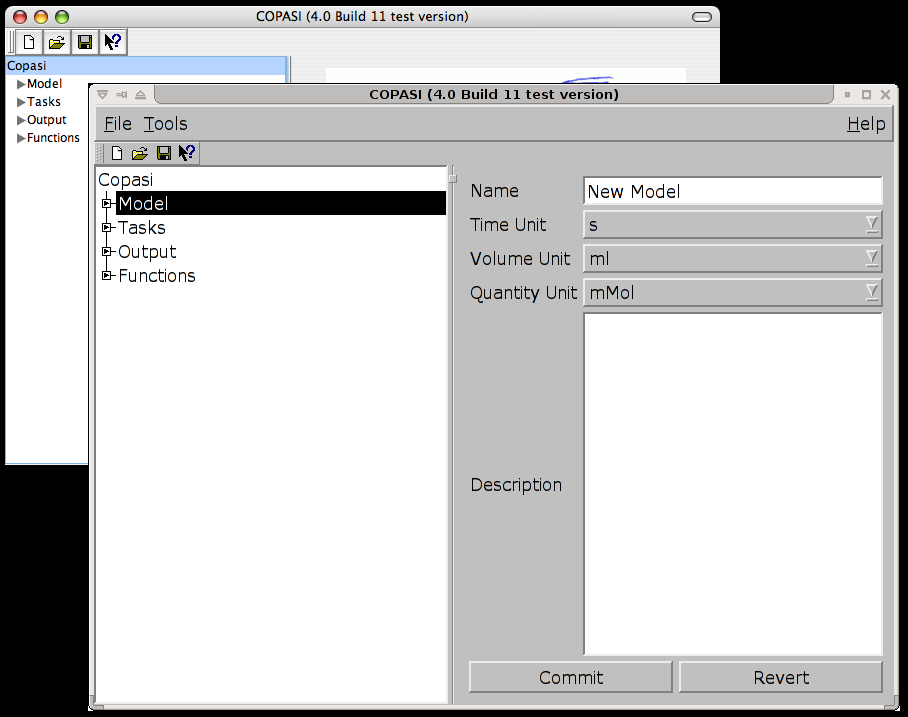
\includegraphics[scale=0.3]{images/Platforms_01.png}}}


It also has the advantage that Copasi essentially behaves the same on all platforms supported, while still showing platform specific behavior. E.g. on a Mac OS X computer, the user will have the menu at the top of the screen and the menu entry for the about dialog will appear in the Copasi menu rather then the help menu.

In the following sections, we will explain how to use the graphical user interface of Copasi. Everything should be applicable to all supported platforms. If there is a difference for some platforms we will try to point that out explicitely.

% ------------------------   
% Section 
\section{Copasi GUI Elements}
\label{generalGUILayout}\hypertarget{generalGUILayout}{}%

The Copasi graphical user interface essentially consists of four elements.


{{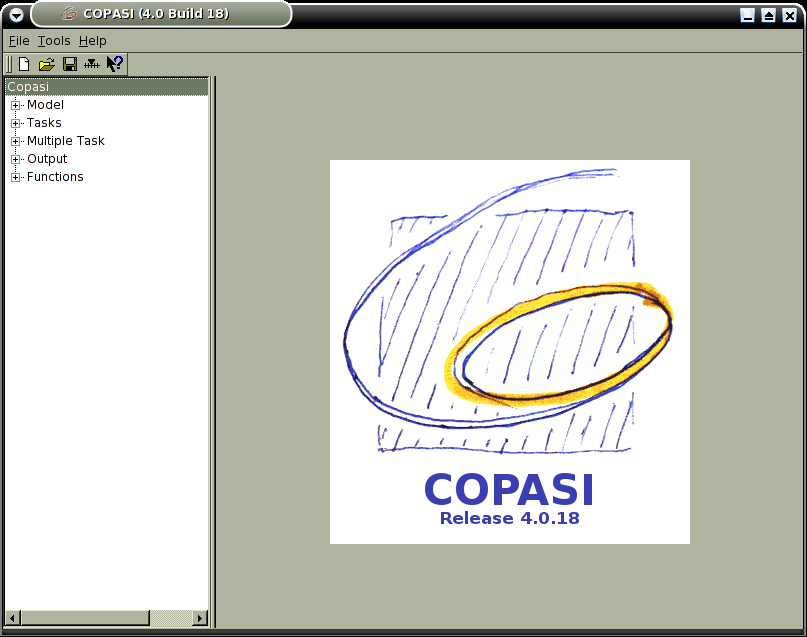
\includegraphics[scale=0.3]{images/Layout_01.png}}}


On the top of the main window, you have the menubar (on the Mac, the menubar is on the top of the screen), below that, you have a toolbar with some common tasks like opening a file or saving a file. The rest of the window is vertically divided into two parts by a slider. The size of the two elements can be adjusted by moving the bar that seperates them. The left element is called the object tree and it shows your current model and the tasks that you can perform on this model. Depending on the element that is selected in the object tree, the view on the right will change in order to enable you to edit the model or run and modify the task you selected in the object tree.

If you start Copasi without any command line argument, Copasi will start with a new model. The root of the object tree will be selected and on the right side of the main window, you will see the Copasi logo.

The object tree has four branches below the root element. The first one contains all objects that belong to the current model. The second one contains all tasks that Copasi can execute, the third one contains the different output objects Copasi can handle and the last branch contains all the (kinetic) functions that are defined. These include the build in functions as well as functions defined by the user.

If you now click on the {\sffamily \bfseries Model} branch, the view to the right of the object tree will change and you will see a screen that allows you to make \hyperlink{generalSettings}{{[model settings]}}. In the following sections, we will escribe the individual dialogs that you can open by selecting different branches in the object tree. During this explanation, you will learn how to create a model in Copasi and run different tasks on this model like calculating a trajectory.

% ------------------------   
% Section 
\section{General Model Settings}
\label{generalSettings}\hypertarget{generalSettings}{}%

If you click on the {\sffamily \bfseries Model} branch of the object tree which was explained in the \hyperlink{generalGUILayout}{{[Copasi GUI Elements]}} section, you activate the dialog that lets you specify certain parameters for your model like its name and the units that are to be used for time, volume and concentration quantities througout the current model. Here you can also give a textual description of you model that is more expressive then reactions and equations. You could for example state which part of the metabolism the model describes (e.g. glycolysis) and add some references to articles related to the model. This will help others (and yourself) to understand and identify your models.


{{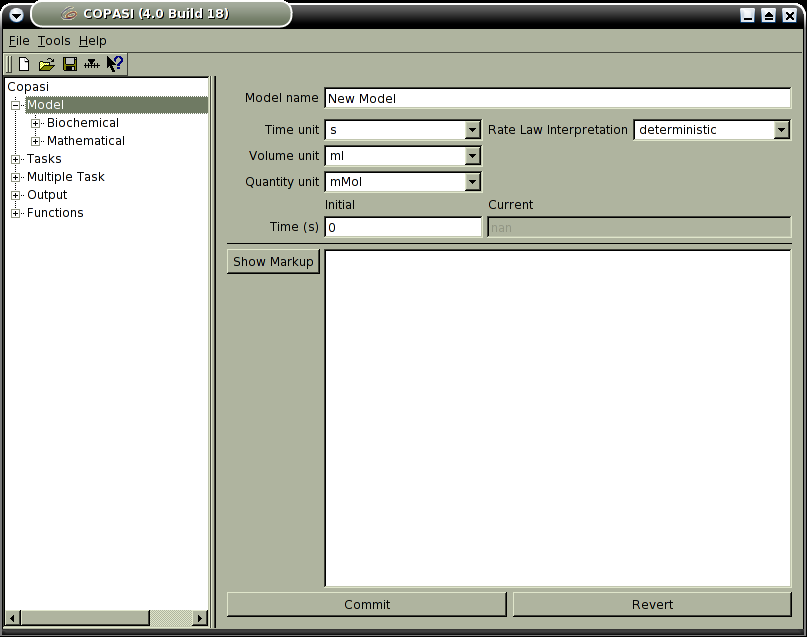
\includegraphics[scale=0.3]{images/General_01.png}}}


% ------------------------   
% Section 
\section{Adding and Editing Compartments}
\label{addingCompartments}\hypertarget{addingCompartments}{}%

In Copasi, most of the time there are several ways to do something and you just choose the way you prefer. This is especially true for defining the elements of the model.

Actually if you are just defining a model that has a single compartment, you will most likely not even bother to add the compartment explicitely, but I will come back to this in the \hyperlink{addingSpecies}{{[Adding and Editing Species]}} and \hyperlink{addingReactions}{{[Adding and Editing Reactions]}} sections.

Although you will probably not add compartments to often, it is good to know how it is done, especially since adding other components of the model, e.g. species or reactions, works essentially the same.

There are three methods to add a new compartment to a model, but for all three, we have to navigate to the {\sffamily \bfseries Compartments} branch of the object tree which is located under the {\sffamily \bfseries Model-\textgreater{}Biochemical} branch. So first open the {\sffamily \bfseries Model} branch and there open the {\sffamily \bfseries Biochemical} branch by clicking on the expansion sign in front of the branch name, or by double clicking on the branch name.


{{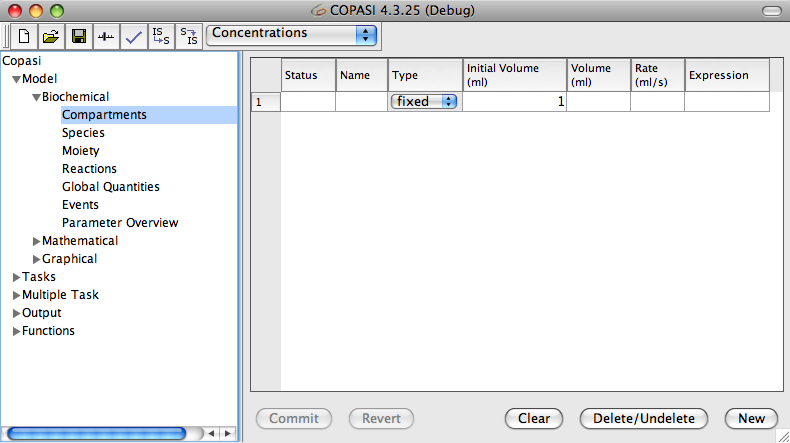
\includegraphics[scale=0.3]{images/Compartments_01.png}}}


If you start with a new model and you select the {\sffamily \bfseries Compartments} branch, you will get an empty table with three columns. The columns are named {\sffamily \bfseries Status}, {\sffamily \bfseries Name} and {\sffamily \bfseries Volume}. {\sffamily \bfseries Name} is the actual name of the compartment and {\sffamily \bfseries Volume} is its volume given in the volume units defined in the \hyperlink{generalSettings}{{[model settings]}} dialog. The meaning of the {\sffamily \bfseries Status} column will be explained shortly.

The most obvious way to add a new compartment is to click the {\sffamily \bfseries New} button on the bottom of the window. This will create a new compartment that is added to the table with a status of {\em{new}}.


{{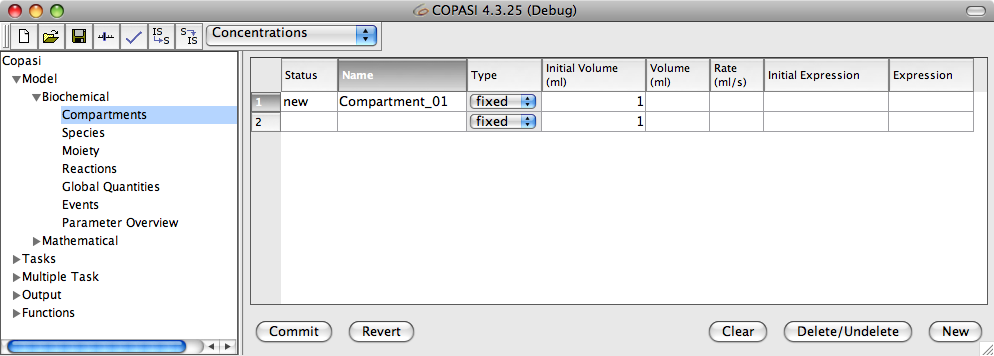
\includegraphics[scale=0.3]{images/Compartments_02.png}}}


A status of new means that the compartment has been created, but is has not been added to the model yet. It will get added to the model if you either click on the {\sffamily \bfseries commit} button on the bottom of the screen, if you selected another element in the object tree on the left, or if you double click on the table. Lets assume you clicked on the {\sffamily \bfseries commit} button, you will notice that the status of the new compartment is no longer defined as new since it has been added to the model.

While the status of a compartment is shown as {\em{new}}, you can remove the compartment from the table by clicking the {\sffamily \bfseries revert} button which will cancel all modifications you made to the compartments that have not been commited yet.


{{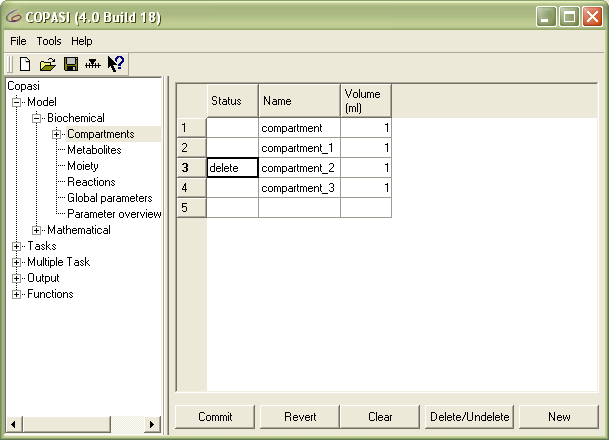
\includegraphics[scale=0.3]{images/Compartments_03.png}}}


If you have already commited the compartment, you can delete it by selecting the table row (or one cell of the table row) that contains the compartment you want to delete and clicking the {\sffamily \bfseries delete} button. You will notice that the compartment does not get deleted at once, but rather the status changes to {\em{deleted}}. You can still undo the delete by clicking the {\sffamily \bfseries revert} button or the {\sffamily \bfseries delete/undelete} button, or you can finalize the delete action by clicking on the {\sffamily \bfseries commit} button. Again leaving this dialog by selecting another object in the object tree or double clicking on the table has the same effect as clicking on the {\sffamily \bfseries commit} button.

The {\sffamily \bfseries clear} button is just a convenience function to delete all compartments. If you click on it, the status of all compartments in the table will be changed to {\em{deleted}} and a subsequent {\sffamily \bfseries commit} will remove the compartments from the model.

The most convenient way to add a compartment is to just click on an empty name cell in the table and type the name of the compartment. Once you leave the cell by either hitting the return or the tab key or by clicking somewhere else, the compartment appears in the table with a status of {\em{new}}. Actually hitting the return key after typing the name brings you directly into the next row and you can continue adding compartments until all compartments are defined. You now only have to commit your changes in one of the ways mentioned above and all the compartments get added to the model.

The third way to add a new compartment is to double click on an empty row in the table. This is essentially the same as clicking the {\sffamily \bfseries new} button and double clicking on the newly added compartment entry.


{{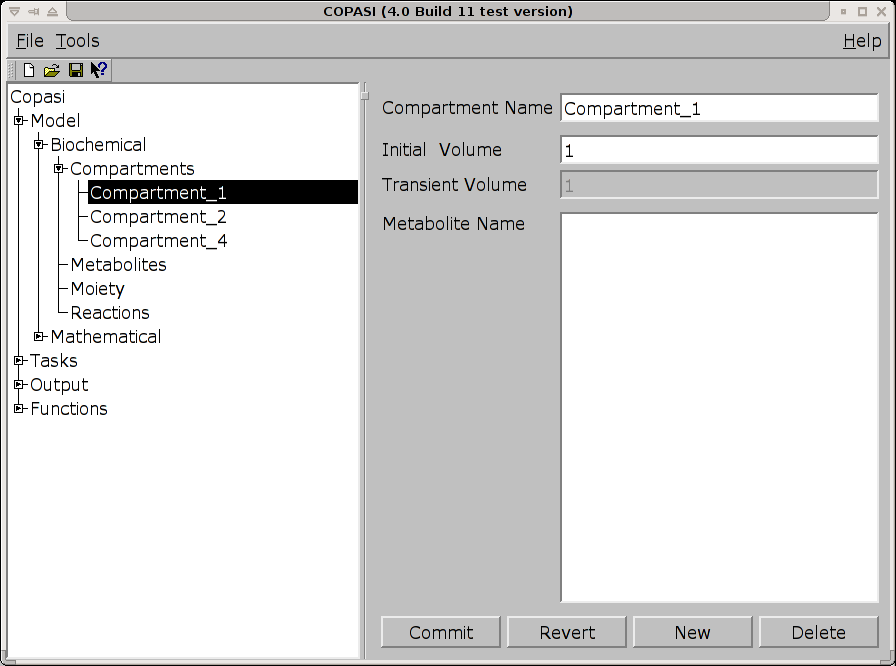
\includegraphics[scale=0.3]{images/Compartments_04.png}}}


Double clicking on any compartment entry in the table will bring you to another input dialog that lets you specify the parameters of the compartment. For a compartment, there are only two parameters that the user can change. One is the name of the compartment and the other is the volume.

If there are already species defined that are part of the compartment being edited, they are listed in the text widget at the bottom of the dialog called "Metabolite Name".

As you might already have noticed, this dialog for changing compartment parameters is associated with the individual compartment leaves in the object tree. So if you want to change the parameters of a compartment, you can also navigate to the leave in the object tree that represents the compartment you want to change instead of double clicking on an entry in the compartment table.

% ------------------------   
% Section 
\section{Adding and Editing Species}
\label{addingSpecies}\hypertarget{addingSpecies}{}%

Adding new species works exactly the same as adding new compartment, so I suggest reading the \hyperlink{addingCompartments}{{[Adding and Editing Compartments]}} section if you haven't already done so. Here we will just cover the differences between adding a compartment and adding a species.


{{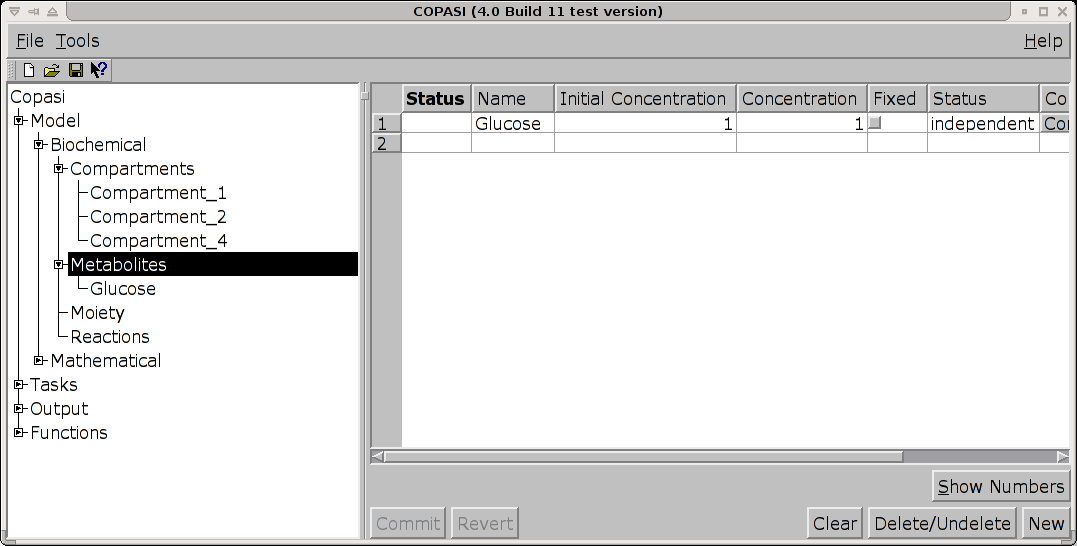
\includegraphics[scale=0.3]{images/Metabolites_01.png}}}


First of all in order to add a new species or metabolite, as it is called in Copasi, you have to navigate to the {\sffamily \bfseries Metabolites} branch of the object tree which is located in the {\sffamily \bfseries Model-\textgreater{}Biochemical} branch directly below the {\sffamily \bfseries Compartments} branch. Here again you see a table, but this table consists of eight columns. This is due to the fact that a metabolite has more parameters than a compartment. The {\sffamily \bfseries Status} and {\sffamily \bfseries Name} columns should already be familiar from the compartments table. The other six columns specify the initial concentration of the metabolite, the transient concentration and if the metabolite is fixed (i.e. its concentration does not change during the course of a simulation). The second {\sffamily \bfseries Status} column might be a litle confusing, but it indicates wether the metabolite is an independent or a dependent metabolite as opposed to the first {\sffamily \bfseries Status} column that indicates wether a metabolite has been added to the model yet or is about to be deleted from the model as described in the \hyperlink{addingCompartments}{{[Adding and Editing Compartments]}} section. The column named {\sffamily \bfseries Compartment} shows the name of the compartment the metabolite belongs to and the {\sffamily \bfseries Rate} column shows the reaction rate of the metabolite. For newly created metabolites the rate will be empty since it needs to be calculated first, e.g. during a \hyperlink{calculatingTrajectory}{time course simulation}.

When a metabolite is added and the model does not contain a compartment yet, Copasi will automatically add a new compartment to the model and the metabolite will be added to this compartment. If there already is one or more compartments, the metabolite will be added to the first compartment in the list. This can be changed later.

To add a new metabolite you have the same three ways as for adding compartments and if you are not familiar with those, I recommend reading the \hyperlink{addingCompartments}{{[Adding and Editing Compartments]}} section.


{{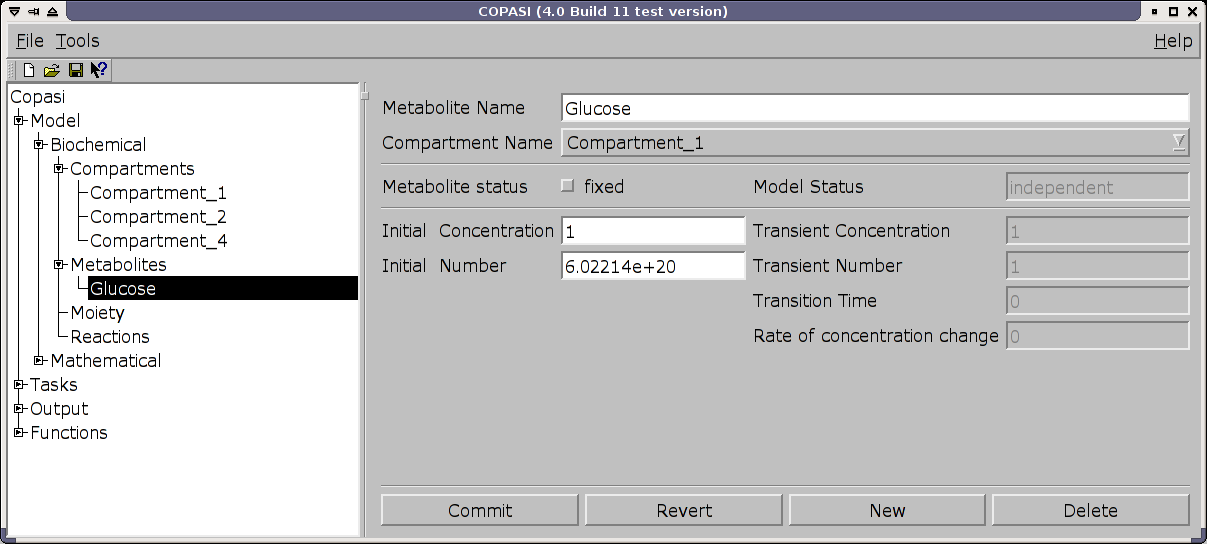
\includegraphics[scale=0.3]{images/Metabolites_02.png}}}


Editing the parameters of a metabolite also works exactly the way it does for compartments. Either you double click on a metabolite entry in the table, or you use the object tree to navigate to the metabolite leave you intend to edit. Some of the parameters of a metabolite like the {\sffamily \bfseries Model Status} are calculated automatically and can not be changed by the user. The parameters that you can change are the {\sffamily \bfseries Name} of the metabolite, the {\sffamily \bfseries Compartment} it belongs to, wether it is a fixed metabolite and its {\sffamily \bfseries initial concentration}. Instead of changing the {\sffamily \bfseries initial concentration}, you can also change the {\sffamily \bfseries initial particle number}. If you change one of those two, the other will be updated automatically. The volume to calculate particle numbers from concentration and vice versa comes from the compartment associated with the metabolite.

% ------------------------   
% Section 
\section{Adding and Editing Reactions}
\label{addingReactions}\hypertarget{addingReactions}{}%

Again adding reactions essentially works the same way as adding compartments or metabolites. When you navigate to the {\sffamily \bfseries Reactions} branch of the object tree which is located under the {\sffamily \bfseries Model-\textgreater{}Biochemical} branch, you will see a table with five columns. The first two are again {\sffamily \bfseries Status} and {\sffamily \bfseries Name} of the reaction. The third column called {\sffamily \bfseries Equation} describes the chemical formula and maybe additional modifiers of the reaction. The fourth column states the name of the kinetics for the reaction which depends on the equation. We will come to this in a second. The last column shows the {\sffamily \bfseries flux} through this reaction. The flux can not be set by the user but is calculated automatically when you \hyperlink{calculatingTrajectory}{do a time course simulation}.


{{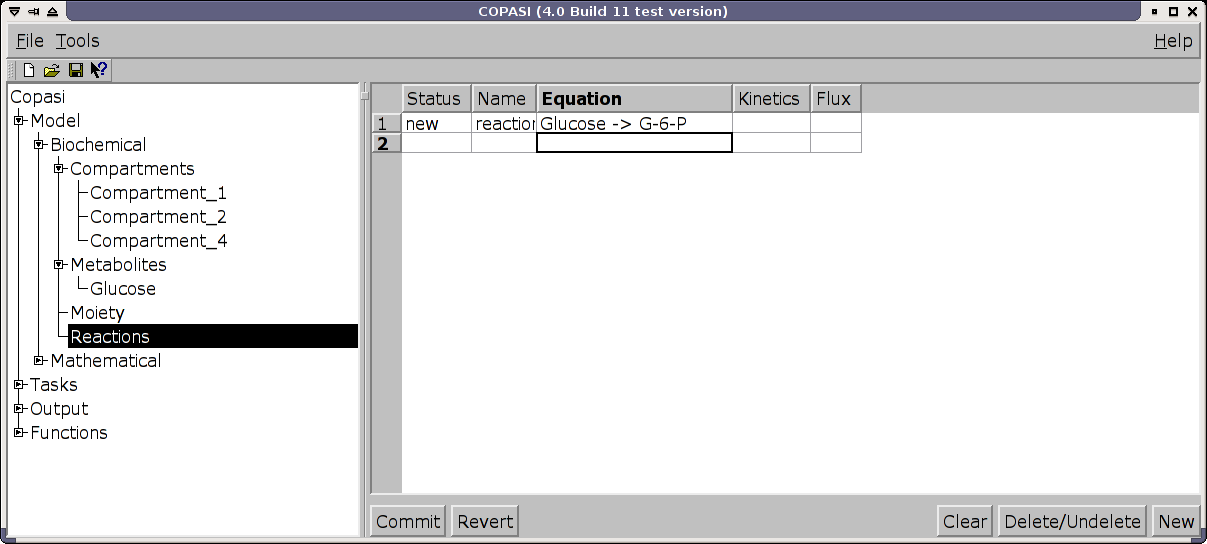
\includegraphics[scale=0.3]{images/Reactions_01.png}}}


The easiest way to add a reaction is to type the chemical equation into an empty equation cell in the table. After you typed the equation, you hit the return key and automatically land in the next row where you can type the next reaction equation. This way you can enter all the reactions that make up your model. When you are finished with typing the reaction equations, you commit all the reactions. If any of the reactions contain metabolites that are not already present in the model, they are added automatically. If there was no compartment before, a compartment is also added and all new metabolites get added to this compartment. If there is already one or more compartment, all new metabolites get added to the first compartment that is listed in the object tree. Each new reaction gets a default kinetic which is irreversible mass action for reactions that contain a substrate. For reaction that only have a product (e.g. influx into a system) a constant flux kinetic is chosen.


{{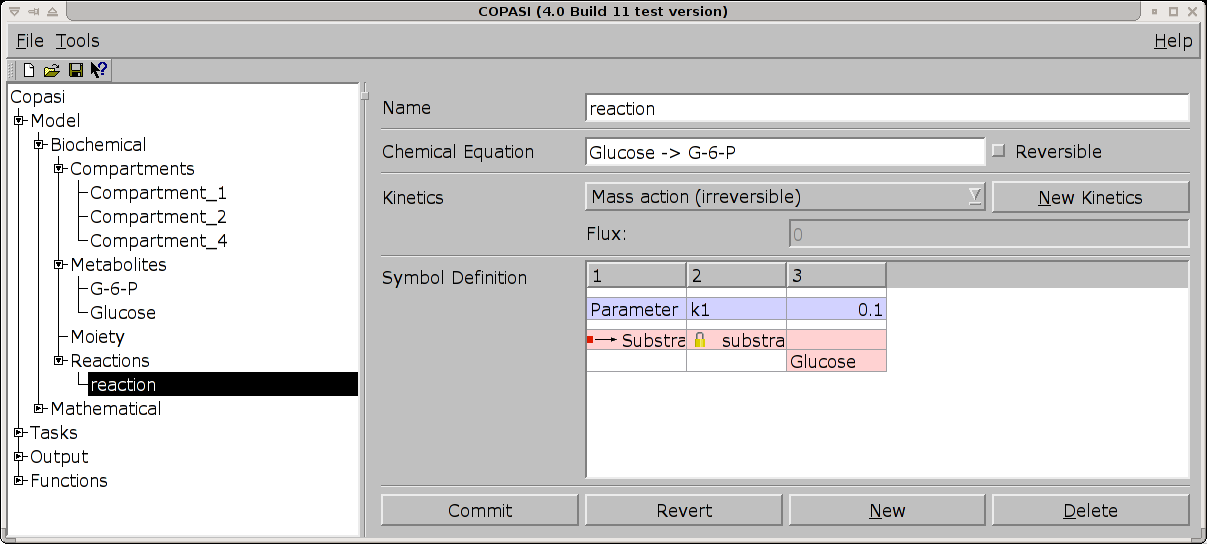
\includegraphics[scale=0.3]{images/Reactions_02.png}}}


Double clicking on an entry in the table will bring you to another dialog that lets you change certain parameters of the reaction. You can change the name of the reaction, the chemical equation and wether the reaction is reversible or not. Changing the chemical equation and the reversibility of a reaction influences the type of kinetics you can choose for the reaction. Each kinetic function defines how many substrates, products and modifiers it expects. Additionally it defines wether it can be used for reversible or irreversible reactions only or if it can be used on either. So depending on how many substrates, products and modifiers your kinetic equation has and wether it is reversible or not, only a subset of the defined kinetic functions will be available in the {\sffamily \bfseries Kinetics} combobox. If the kinetic function you want to assign to the reaction is not available yet, you can add it by clicking on the {\sffamily \bfseries New Kinetics} button (see also \hyperlink{addingFunctions}{{[Adding and Editing User Defined Functions]}}). Depending on the kinetic function you chose, you get a selection of parameters in the table named {\sffamily \bfseries Symbol Definition}, all functions parameters get a default value of 0.1 which can be changed by clicking into the corresponging cell and typing a new value.

So far we did not go into the details of how chemical equations are to be specified. Chemical equations have a simple schema. First you state all the substrates seperated by "+" characters. Please make sure that you seperate the name of the substrate and the "+" character by at least one space character, otherwise Copasi will interpret the "+" sign as belonging to the metabolites name. (Having the "+" character as part of a metabolites name is allowed in Copasi!) after the list of substrates, you specify either an equals ("=") character if the reaction is reversible or the character combination "-\textgreater{}" if the reaction is irreversible. This is followed by the list of products which must also be seperated by the "+" character. Again make sure you have spaces around the seperating "+" characters. Optionally this term can be followed by a semicolon and a list of modifiers which are comma seperated. Either the list of substrates or the list of products may also be empty, but at least one of them must be present. Lets look at two examples: 
\begin{enumerate}[a]
%--- Item
\item 
Metabolite A is irreversibly converted into Metabolite B. The chemical equation you would type is "A -\textgreater{} B".


%--- Item
\item 
Metabolite A and B are reversibly converted to Metabolite C, the reaction has to modifiers C and D. The chemical equation for this in Copasi would be: "A + B = C; C,D"

Note that one of the modifiers is the product!

\end{enumerate}
\noindent 

% ------------------------   
% Section 
\section{Definining Output}
\label{outputDefinitions}\hypertarget{outputDefinitions}{}%

After you have \hyperlink{addingReactions}{defined all reactions} that make up your model, you could go ahead and do some calculations with your model. For some of the task this is fine since they show you the results in a seperate results dialog and it might not be necessary to store those into a file. For other tasks like e.g. a time course, it is very likely that you would like to store the resulting trajectory in some file or plot the result for visual inspection. So if you want Copasi to store the results or do a plot of them, you have to define either a report and associate it with a file or define a plot. (In the \hyperlink{calculatingTrajectory}{{[Running a Time Course Simulation]}} section we will also offer an alternative, albeit less flexible, way for storing the results of a time course simulation.)
\subsection{Defining Reports}
\label{reportDefinitions}\hypertarget{reportDefinitions}{}%


{{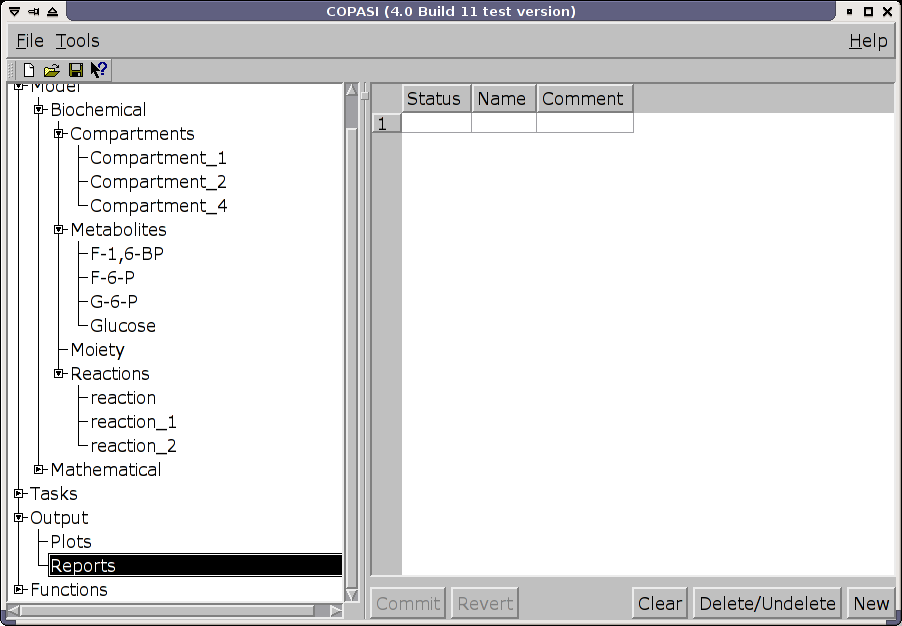
\includegraphics[scale=0.3]{images/Reports_01.png}}}


The dialog for defining report definitions is located under the {\sffamily \bfseries Output-\textgreater{}Reports} branch in the object tree. Double clicking on an empty row in the table creates a new report object and opens the dialog for modifying the report definition. In this dialog, can can specify a name for the report in the {\sffamily \bfseries ReportDefinition} field. In the {\sffamily \bfseries task} combobox, you can choose for which kind of task this report should be written, so if you want to store the result of a time course, you choose {\em{Trajectory Task}} here. The report usually stores the results of its task as a table; the standard separator character for elements in this table is the tab character (\textbackslash t). If you want to change this, you have to uncheck the Tab checkbox and specify the separator character or string you want in the {\sffamily \bfseries Separator} field.  Next you have to define the objects that you want to appear in the report. To add a new object to the report definition, you have to click on the button with the {\sffamily \bfseries +} symbol. This will open the object browser dialog.


{{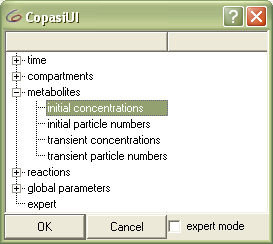
\includegraphics[scale=0.3]{images/Reports_02.png}}}


The object browser dialog shows a tree of all the objects that are known to Copasi. The objects that belong to your model are located in the branch that corresponds to the name of your model. The position of that branch varies since the branches are sorted alphabetically. Each branch and leave in the object browser has a check box in front of its name. This checkbox can have three states. The unchecked state means that no object in this subtree are selected. A checkmark on a black background means that the whole subtree is selected, i.e. all objects in this subtree are selected. A checkmark on a gray background means that part of the subtree is selected.


{{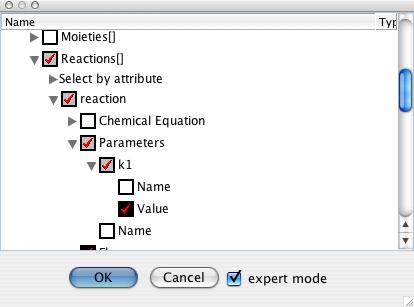
\includegraphics[scale=0.3]{images/Reports_03.png}}}


Due to the model structure, most objects appear more than once in the tree. So if you select some object, you should not be surprised, if more than the selected object suddenly change their selection state. E.g. if you select the whole {\sffamily \bfseries Compartments} subtree of your model, all the metabolites which are part of the compartments get selected as well which means that on selecting the {\sffamily \bfseries Compartments} branch, the whole {\sffamily \bfseries Metabolites} branch changes its state to selected.

Lets assume you want to define the report for a trajectory task. In this case, you will probably want the time and some or all of the transient concentration of the metabolites in your report. The time for the time course is the last item in the model branch, you select it by clicking on the check box in front of the name. If you want to add the concentrations of all metabolites, you open the {\sffamily \bfseries Metabolites} subbranch in the {\sffamily \bfseries Model} branch and open the {\sffamily \bfseries Select by attribute} branch. There you can select the {\sffamily \bfseries Concentration} attribute. Selecting the {\sffamily \bfseries Concentration} attribute will select the concentrations for all metabolites. If you only want to have some of the metabolites in your report, you open the subbranches of the metabolites you want in the {\sffamily \bfseries Metabolites} branch and select the {\sffamily \bfseries Concentration} attribute only for those metabolites. If your model contains many metabolites and you want to have all but one or in your report, it is often easier to first select all concentrations via the {\sffamily \bfseries Select by attribute} branch and then deselect the ones you don't want, rather then selecting the individiual concentration you want. Once you are finished with selecting the objects for your report, you confirm the selection by clicking the {\sffamily \bfseries OK} button in the object browser. The objects you selected will now appear in the listbox of the report definition dialog.


{{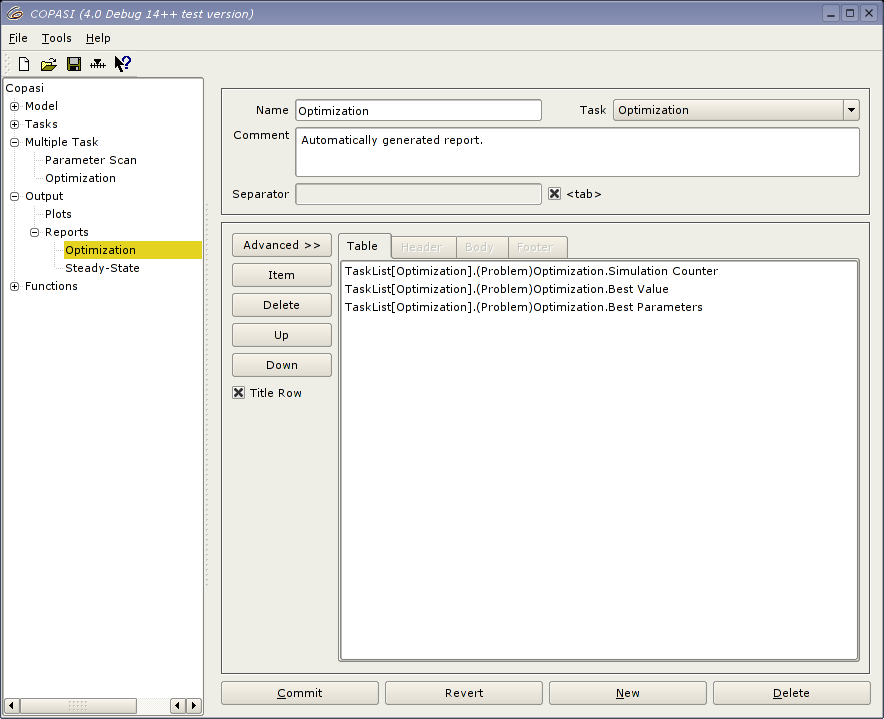
\includegraphics[scale=0.3]{images/Reports_04.png}}}


They will appear in the report in the same order as they appear in this list. To reorder the entries in the list, you can select individual entries and move them up and down in the list with the arrow buttons that are located to the left of the list. For example it might be a good idea to move the time object to the top of the list so that it will appear as the first table column in the file since this is the way most programs would expect it. The only thing that is now left is to connect this report to a file. This has to be done in the dialog for the specific task and we will cover this when we explain how to run the individual tasks.
\subsection{Defining Plots}
\label{plotDefinitions}\hypertarget{plotDefinitions}{}%

Plotting is another form of output that Copasi can do. So far plotting is limited to the results of a \hyperlink{calculatingTrajectory}{time course analysis} but plotting of other results will eventually be available where it makes sense. Most of the time, you probably want to plot some or all of the metabolites concentrations during a time course simulation.


{{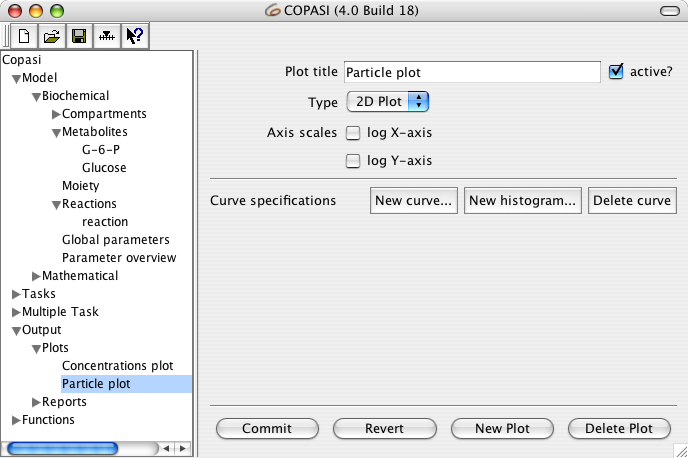
\includegraphics[scale=0.3]{images/Plots_01.png}}}


To define a plot, you open the plot definition dialog which you reach by selecting the {\sffamily \bfseries Output-\textgreater{}Plots} branch in the object tree. If you intend to plot all or most of the metabolites concentrations agains the time, the easiest way to define this plot is to click on the {\sffamily \bfseries Add default plot} button on the bottom of the dialog. This creates a plot with all concentrations against the time. If this is OK, you are done. If you want to remove some of the concentrations, you edit the plot by double clicking on the plot entry in the table, or by selecting the new plot definition in the object tree. A plot in Copasi is made up of a number of curve objects. For each curve, there is a tab in the plot definition dialog. To remove one of the curves, you have to select the tab that corresponds to the curve you want to remove and then click on the {\sffamily \bfseries Delete Curve} button. The next time you do a \hyperlink{calculatingTrajectory}{time course simulation}, each plot that is marked as active will be plotted automatically. How you define a plot as being active will be explained in the next paragraph. If you want to plot something other then the concentrations of the metabolites, e.g. the particle numbers against the time, you have to define your own plot. To do this, double click on an empty row in the plot table. (You get to the plot table by selecting the {\sffamily \bfseries Output-\textgreater{}Plots} branch in the object browser.)


{{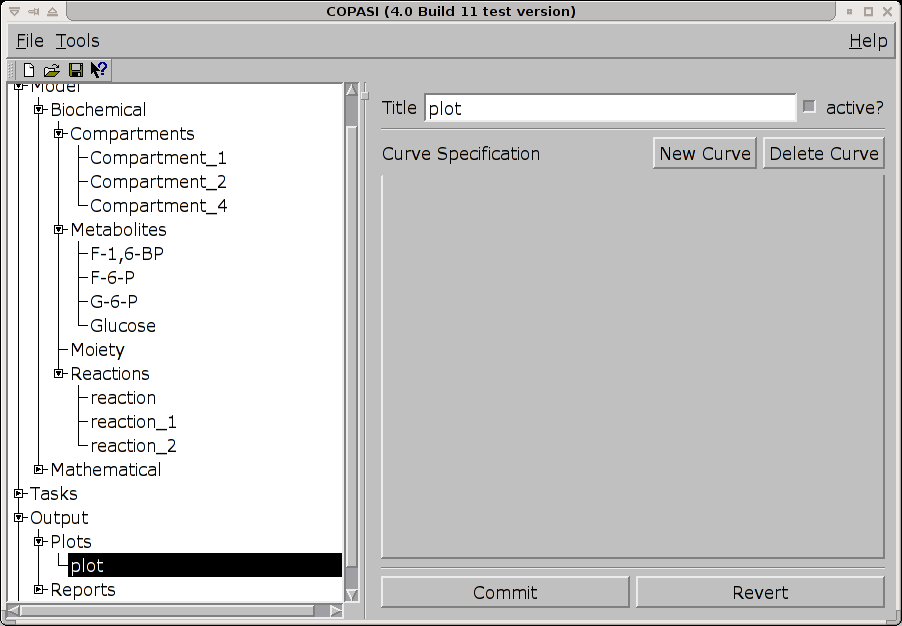
\includegraphics[scale=0.3]{images/Plots_02.png}}}


This opens a plot definition dialog that contains no curves. If you want to add a curve, you click on the {\sffamily \bfseries New Curve} button. A selection dialog opens that lets you choose an object for the x axis and one or more objects for the y axis. The tree on the left is a single selection tree which lets you choose the object that defines the x axis of the plot. Most often this will be the time. So if you want the time to be drawn on the x axis, select the time leave in the {\sffamily \bfseries Time} branch. The right tree is a multi selection tree where you can choose one or more elements to be drawn on the y axis. There you could e.g. choose all transient particle numbers.


{{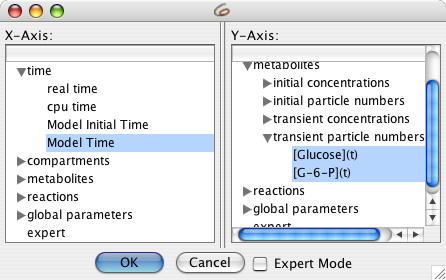
\includegraphics[scale=0.3]{images/Plots_03.png}}}



{{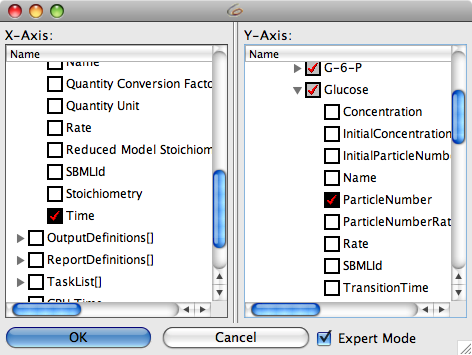
\includegraphics[scale=0.3]{images/Plots_04.png}}}


In order to select objects in the multi selection tree, you select them in the tree and push the add button on the right of the selection dialog. The selected objects will show up in the listbox beside the tree. If you want to select more objects, select them in the tree and push the {\sffamily \bfseries Add} button again. You can do this as often as you like, but each object can only be selected once. All objects that are already marked as selected, i.e. that appear in the listbox, are disabled in the tree and can not be added a second time. On the other hand, if you want to remove some of the objects that you have selected, select them in the list and push the {\sffamily \bfseries Delete} button. You can also reorder the items in the list with the {\sffamily \bfseries Move Up} and {\sffamily \bfseries Move Down} buttons. (This is not needed for plots!) The trees in this dialog only have a limited set of the total objects that you e.g. see in the \hyperlink{reportDefinitions}{object browser}. If the object you want to plot is not in this simplified tree, you can check the {\sffamily \bfseries Expert Mode} checkbox on the bottom of the dialog. This will give you two full \hyperlink{reportDefinitions}{object browser} trees from which you can select objects.


{{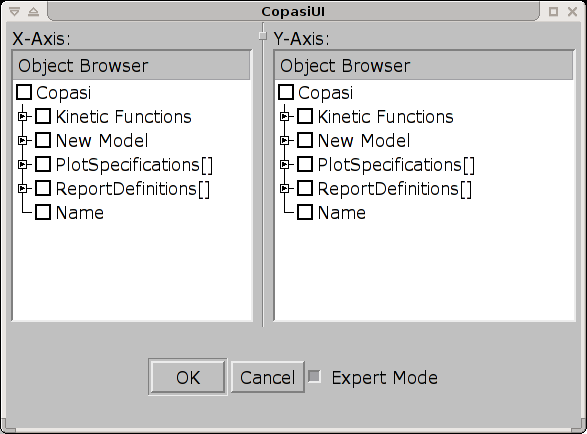
\includegraphics[scale=0.3]{images/Plots_05.png}}}


Once you are finished with your selection, you confirm your selection with the {\sffamily \bfseries OK} button. Copasi now creates a curve object for each object you selected for the y axis and adds it to the plot. Each curve is represented as a tab in the plot definition dialog. 
\begin{admonition}{figures/caution}{Attention}% NOTICE: see the db2latex FAQ w.r.t db2latex variable $latex.admonition.path

On Mac OS X, the tab widget does not handle very wide tabs or many tabs well. This problem will be dealt with in upcoming versions of Copasi.
\end{admonition}



In the plot definition dialog, in addition to adding and removing curve objects, you can specify a name for the plot definition and you can specify wether the plot should be active or not with the {\sffamily \bfseries active} checkbox. (Only plots that are active are drawn when a \hyperlink{calculatingTrajectory}{time course simulation} is run!)

Another way to specify wether a plot is active or not is in the plot table where all the plots are listed. Each row in the table contains a column named {\sffamily \bfseries active} that contains a checkbox with which you can toggle the state of a plot. If you changed the state of one or more plots, you have to commit these changes either by clicking the {\sffamily \bfseries Commit} button or any other action that is equivalent to pressing the {\sffamily \bfseries Commit} button (see \hyperlink{addingCompartments}{{[Adding and Editing Compartments]}} section).

% ------------------------   
% Section 
\section{Adding and Editing User Defined Functions}
\label{addingFunctions}\hypertarget{addingFunctions}{}%

Copasi already defines a rather large set of common kinetic functions to choose from. Nevertheless sometimes you will have to define your own kinetic function to solve a specific problem. The list of defined functions is located as the last branch in the object tree.


{{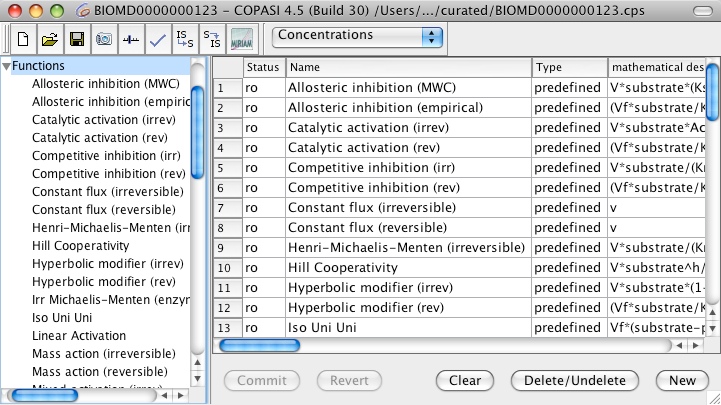
\includegraphics[scale=0.3]{images/Functions_01.png}}}



{{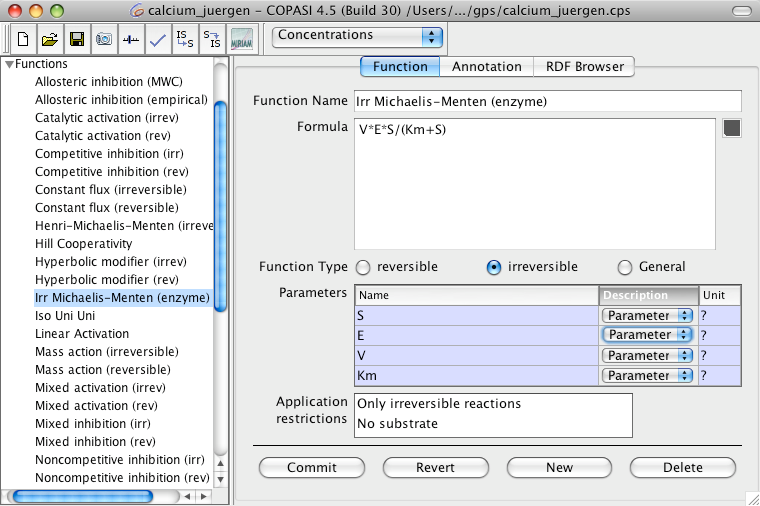
\includegraphics[scale=0.3]{images/Functions_02.png}}}


You can add a new function either by double clicking on an empty table row or by clicking on the {\sffamily \bfseries new} button on the bottom of the screen. In the function definition dialog, you give your function a name in the {\sffamily \bfseries Function Name} field. This name has to be unique within the list of defined functions. Next, you have to specify a formula that defines the reaction rate of your kinetic function in the {\sffamily \bfseries Formula} field. The function string only covers the right side of the rate function. So for Michaelis-Menten which is defined as   \begin{displaymath}{{v}{{V}*{ {\left( {{S}/{ {\left( {{K}_{{m}}+{S}} \right)} }} \right)} }}}\end{displaymath}%
  you would enter   \begin{displaymath}{{V}*{ {\left( {{S}/{ {\left( {{K}_{{m}}+{S}} \right)} }} \right)} }}\end{displaymath}%
  into the {\sffamily \bfseries Formula} field. While you are typing the formula, Copasi already tries to parse the equation and extract the parameters. All parameters Copasi finds are listed in the {\sffamily \bfseries Parameters} table below the {\sffamily \bfseries Formula} field. Per default, all variables found are defined as being {\em{Parameters}}. You have to specify which of them really are parameters and which are substrates, products or modifiers. This mapping of variable names to a specific function within the equation also defines the type of reactions this function can be used for. E.g. if you define your function to contain two substrates and a modifier, you can later only use it for functions that really do have two substrates. 
\begin{admonition}{figures/note}{Note}% NOTICE: see the db2latex FAQ w.r.t db2latex variable $latex.admonition.path

The reaction doesn't have to have an explicit modifier since one of the substrates could be a modifier as well!
\end{admonition}

 You can also see this in the {\sffamily \bfseries Application} table below the {\sffamily \bfseries Parameters} table. Lets say you define the function   \begin{displaymath}{{A}*{B}}\end{displaymath}%
  and define {\em{A}} and {\em{B}} to be substrates, you will see the number 2 in the {\sffamily \bfseries Min} column of the {\sffamily \bfseries SUBSTRATES} row in the {\sffamily \bfseries Application} table. After defining this function, you will be able to use it for all chemical reaction that have at least two substrates. If you would like to limit the maximum number of substrates to lets say four, you would have to set the {\sffamily \bfseries Max} column of the {\sffamily \bfseries SUBSTRATES} row to 4. Last but not least you have to define wether this function can be applied to reversible, irreversible or both reaction types by selecting the {\sffamily \bfseries reversible}, {\sffamily \bfseries irreversible} or {\sffamily \bfseries General} radio button respectively. After you commit the function, you can use it for the definition of reactions.

 The operators and functions that Copasi knows and therefore can be used to create user defined functions are the following: 
% table ------------------------------------------------------
\begin{table}[htb]
\begin{center}%
\hypertarget{id2521779}{}%
\captionswapskip{}{{\caption{Mathematical Operators and Functions}\label{id2521779}}}
\captionswapskip{}\begin{tabular}{|l|l|}
\hline 
{{Operator/Function}} & {{Description}} \tabularnewline
 \hline 
{{log / LOG}} & {{natural logarithm}} \tabularnewline
 \hline 
{{log10 / LOG10}} & {{logarithm for base 10}} \tabularnewline
 \hline 
{{exp / EXP}} & {{exponent function}} \tabularnewline
 \hline 
{{sin / SIN}} & {{sine function}} \tabularnewline
 \hline 
{{cos / COS}} & {{cosine function}} \tabularnewline
 \hline 
{{+}} & {{plus operator}} \tabularnewline
 \hline 
{{-}} & {{minus operator}} \tabularnewline
 \hline 
{{/}} & {{division operator}} \tabularnewline
 \hline 
{{*}} & {{multiplication operator}} \tabularnewline
 \hline 
{{\textasciicircum{}}} & {{power function}} \tabularnewline
 \hline 
{{()}} & {{paranthesis for grouping of elements}} \tabularnewline
\hline 
\end{tabular}
\end{center}
\end{table}

 
\begin{admonition}{figures/note}{Note}% NOTICE: see the db2latex FAQ w.r.t db2latex variable $latex.admonition.path

Basic function names can be written with either all lowercase letters or all letters uppercase. Mixing of upper and lowercase letters is not allowed and will lead to errors.
\end{admonition}




\begin{admonition}{figures/caution}{Attention}% NOTICE: see the db2latex FAQ w.r.t db2latex variable $latex.admonition.path

Nesting of function definitions is not possible. A function definition may not contain any other defined functions, only the basic operators and functions listed in the table above.
\end{admonition}



% ------------------------   
% Section 
\section{Doing a Steady State Analysis}
\label{steadyStateAnalysis}\hypertarget{steadyStateAnalysis}{}%

In order to run a steady state analysis, you have to navigate to the {\sffamily \bfseries Task-\textgreater{}Steady-State} branch in the object tree.


{{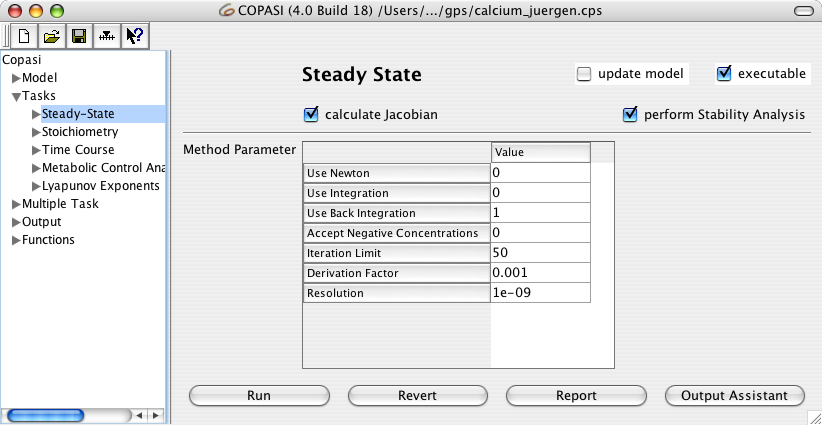
\includegraphics[scale=0.3]{images/SteadyStateTask_01.png}}}


In the dialog that appears there, you can make several settings that influence the way the steady state analysis is calculated. First of all, you can decide wether Copasi should calculate the Jacobian matrix and/or do a stability analysis as well by checking the corresponding checkbox. The {\sffamily \bfseries task executable} checkbox in non functional and can be ignored. In the {\sffamily \bfseries Parameter value} table you can also make several settings that influence the method for calculating the steady state itself. For a detailed description of those parameters will eventually by available in the corresponding methods part of this documentation. To finally run the steady state calculation, click on the {\sffamily \bfseries run} button at the bottom of the screen. After the calculation, Copasi will jump to the results widget.


{{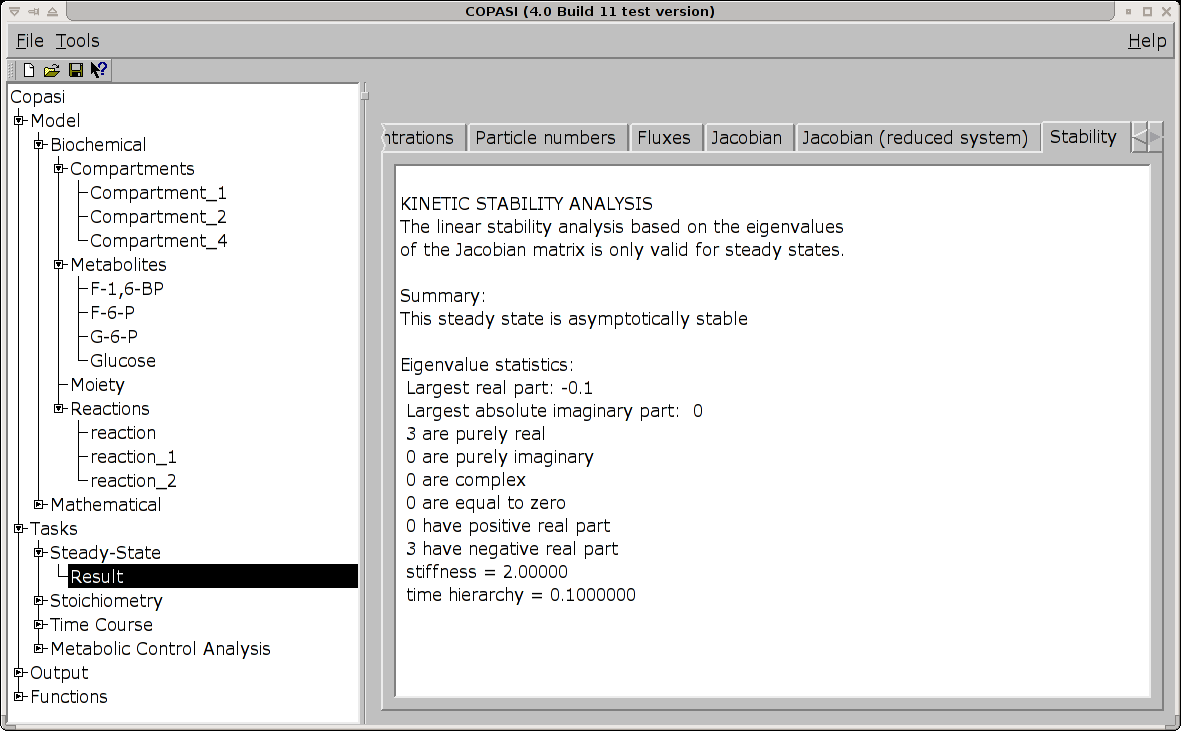
\includegraphics[scale=0.3]{images/SteadyStateTask_02.png}}}


The results widget for the steady state calculation contains several tabs for the individual results. The first and the second tab contain the concentrations and the particle number at the steady state respectively. The third tab contains the fluxes for the reactions at the steady state. It contains concentration fluxes as well as particle fluxes. The fourth and fifth tab only contain results if you told Copasi to calculate the Jacobian matrix. The fourth tab then shows the Jacobian for the full system and the fifth tab contains the Jacobian matrix for the reduced system. The sixth and last tab contains the results for the stability analysis if a stability analysis was requested.

% ------------------------   
% Section 
\section{Elementary Modes and Mass Conservation}
\label{stoichiometryStateAnalysis}\hypertarget{stoichiometryStateAnalysis}{}%
\subsection{Calculating Elementary Modes}
\label{elementaryModes}\hypertarget{elementaryModes}{}%

Letting Copasi calculate the elementary modes for the system is very easy. Select the {\sffamily \bfseries Tasks-\textgreater{}Stoichiometry-\textgreater{}Elementary Modes} in the object tree and click on the {\sffamily \bfseries run} button in the dialog that appears.


{{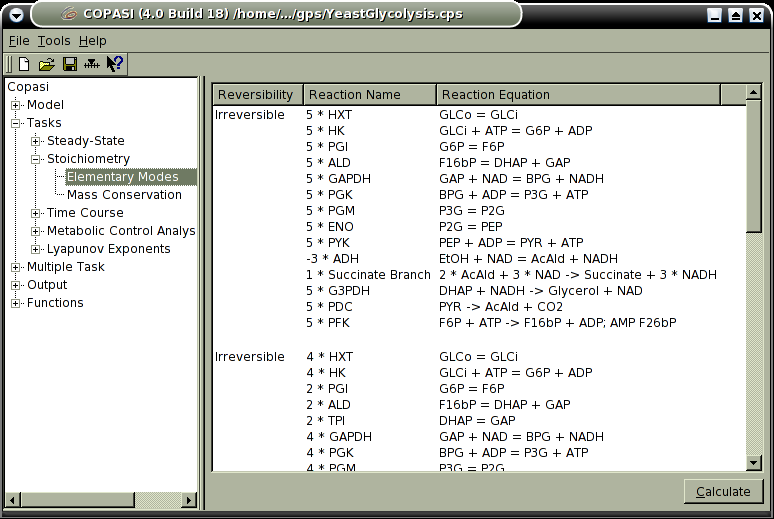
\includegraphics[scale=0.3]{images/ElementaryModesTask_01.png}}}


The elementary modes found will be displayed directly in this dialog. Each elementary mode lists the reactions it consists of together with their chemical equations.
\subsection{Calculating Mass Conservations}
\label{massConservation}\hypertarget{massConservation}{}%

Calculating mass conservations in Copasi is also very easy. Navigate to the {\sffamily \bfseries Tasks-\textgreater{}Stoichiometry-\textgreater{}Mass Conservation} branch in the object tree and click on the {\sffamily \bfseries recalculate} button.


{{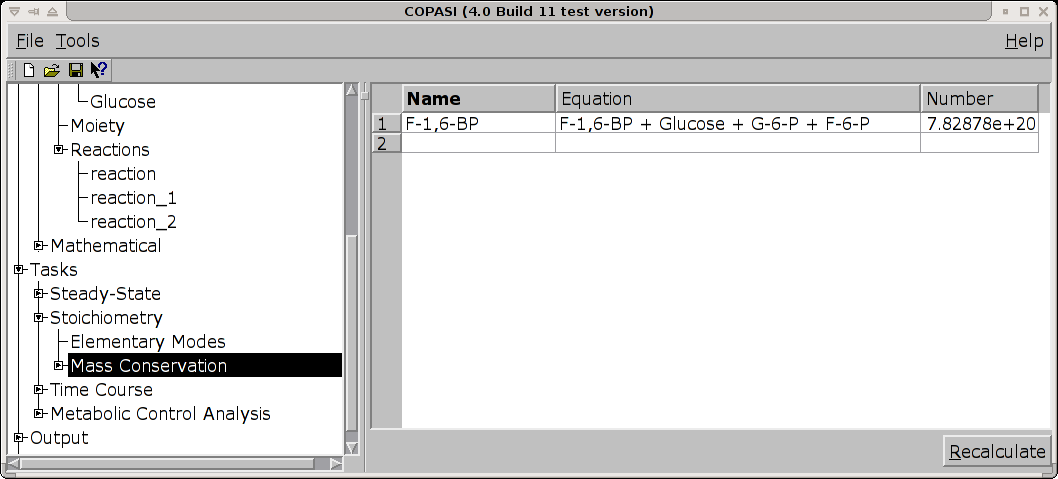
\includegraphics[scale=0.3]{images/MassConservationTask_01.png}}}


If the model contains any mass conservation relations they will be listed in a table directly in this dialog.


{{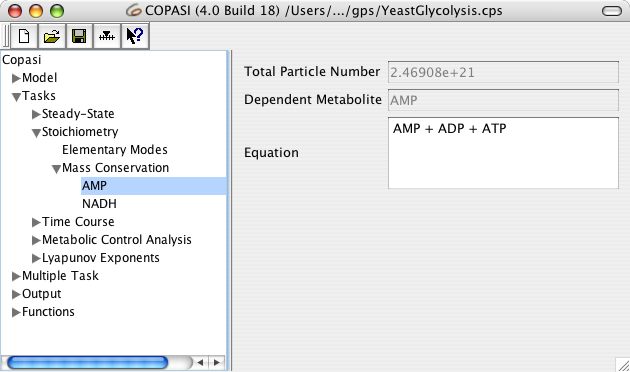
\includegraphics[scale=0.3]{images/MassConservationTask_02.png}}}


Every mass conservation relation also has a separate leave in the object tree below the current dialog. To see those, either navigate there in the object tree or double click on the entry in the table.

% ------------------------   
% Section 
\section{Running a Time Course Simulation}
\label{calculatingTrajectory}\hypertarget{calculatingTrajectory}{}%

To do a time course simulation, you have to navigate to the corresponding task branch in the object tree which is located at {\sffamily \bfseries Tasks-\textgreater{}Time Course}.


{{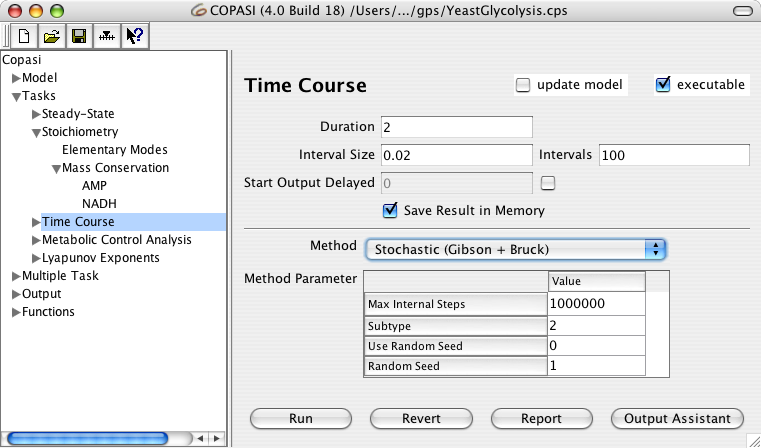
\includegraphics[scale=0.3]{images/TimeCourseTask_01.png}}}


The dialog should be more or less self explaining. You can change several parameters for the time course, e.g. the start time, the end time and the number of intervals that is being calculated in the time range. Alternatively to setting the number of intervals, you can also set the size of the interval. If you set either one, the other will be updated accordingly. Also if you change the time range, number number of intervals will stay the same which means that the interval size will be adjusted. The checkbox labeled {\sffamily \bfseries store time series in memory} tells Copasi to keep the result of the time series calculation in memory in order to display it in a result dialog. Since this can be a large amount of data depending on the size of your model and/or the number of intervals you want Copasi to calculate, you should disable this if you think the result might not fit into memory. The consequence of disabling this checkbox is that you need to \hyperlink{reportDefinitions}{define a report} in order to store the results of the time course simulation.

Copasi supports two different methods for calculating time course simulations. Copasi can use the LSODA solver to calculate the time course deterministicaly or it can use a stochastic solver which uses the {\em{Direct Method}} by Gillespi to calculate the time course stochastically. Depending on the solver you have chosen, you can set several parameters in the {\sffamily \bfseries Parameter value} table that influence the way the method works. A detailed explanation of those parameters will follow in the methods part of this document.

In case you \hyperlink{reportDefinitions}{defined a report definition}, you have to associate this report definition with a file for Copasi to be able to write the results to that file. To do that, you click on the {\sffamily \bfseries Report Definition} button. If no report definition had been defined, Copasi informs you that it created a new one and asks you if you want to edit it. If you don't know how to define a report definition, please go back to the \hyperlink{reportDefinitions}{{[Defining Reports]}} section. Since the report definition Copasi created automatically will be empty, it is recommended that you edit it in order to get some output. Once you are finished creating the report definition go back to the time course dialog and click on the {\sffamily \bfseries Report Definition} button again.


{{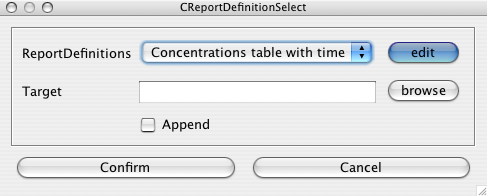
\includegraphics[scale=0.3]{images/TimeCourseTask_02.png}}}


The dialog that pops up will let you choose the report you want to use (in case you created more then one) and lets you browse for a file to store the report to. Additionally, you can choose wether you want to append the report to an already existing file. The default is to create a new file, or to overwrite an existing file. If you want to append to the selected file, you have to check the {\sffamily \bfseries Append} checkbox.

Once you made all the desired changes to the parameters, you can start the time course simulation by clicking on the run button. Copasi will show a progressbar while running the simulation which might take some time depending on several factors like the hardware you are using, the simulation method you chose and/or the size of your model. Once Copasi finishes the calculation, you will find the results in the report file you defined and/or in a seperate result dialog if you told Copasi to keep the results in memory.


{{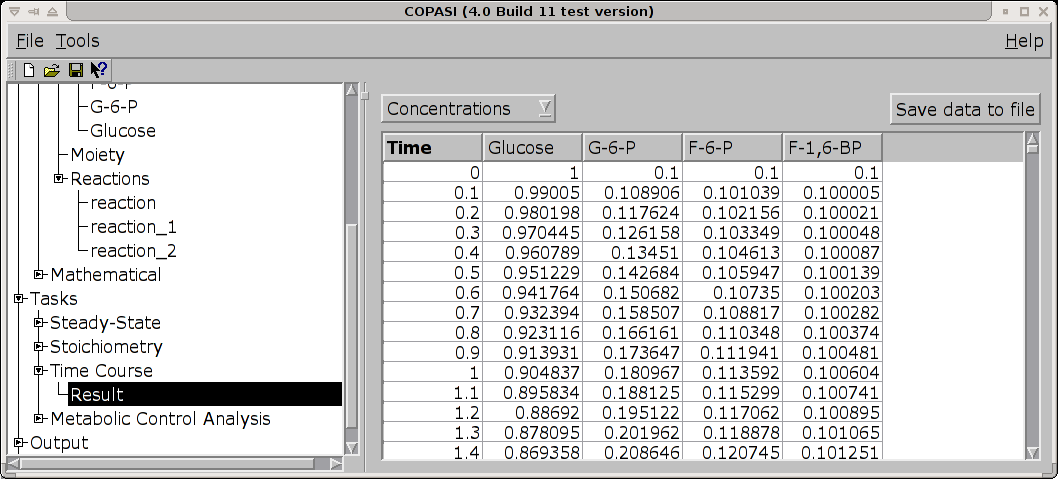
\includegraphics[scale=0.3]{images/TimeCourseTask_03.png}}}


The results dialog is located directly below the time course branch in the object tree. In this widget you can choose wether you want the results to be displayed as concentrations or as particle numbers and you have the possibility to store the results to file. The advantage a report has over writing a file in the results widget is that you can choose exactly which metabolite concentrations you want to store whereas the results dialog always stores all metabolites concentrations.
\subsection{Working with Plots}
\label{workingWithPlots}\hypertarget{workingWithPlots}{}%

If you have an active plot defined while calculating a trajectory Copasi will draw the plot. The plot window has three elements. A toolbar at the top, that lets you zoom into the plot or print the plot. The actual plot and a legend at the bottom. The legend at the bottom is interactive and drawing of certain curves can be toggled by clicking on the corresponding legend entry.

In order to zoom further into a plot, you have to activate the zoom function by clicking on the {\sffamily \bfseries zoom} button in the toolbar at the top of the screen. Once this function is active, you can select a rectangluar area on the plot by clicking somewhere in the plot and dragging the pointer. The plot will now zoom into the area you just selected. To go back to the original plot, right click on the plot area. 
\begin{admonition}{figures/note}{Note}% NOTICE: see the db2latex FAQ w.r.t db2latex variable $latex.admonition.path

Macintosh users with single button mice use CTRL-click.
\end{admonition}



\begin{admonition}{figures/caution}{Attention}% NOTICE: see the db2latex FAQ w.r.t db2latex variable $latex.admonition.path

The qwt plot widget has some problems under Mac OS X. Especially zooming often leads to strange artifacts.
\end{admonition}



{{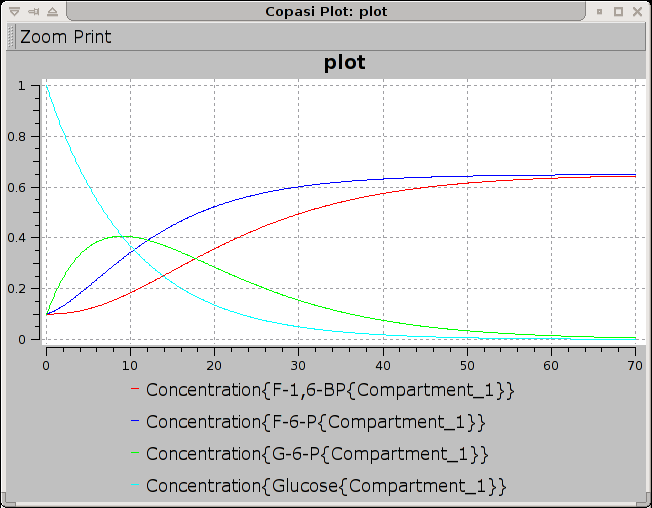
\includegraphics[scale=0.3]{images/PlotWindow_01.png}}}


% ------------------------   
% Section 
\section{Doing a Metabolic Control Analysis (MCA)}
\label{calculatingMCA}\hypertarget{calculatingMCA}{}%

Starting with Build 11, Copasi can calculate the Metabolic Control Analysis (MCA) for your model. The MCA task is located under {\sffamily \bfseries Tasks-\textgreater{}Metabolic Control Analysis}.


{{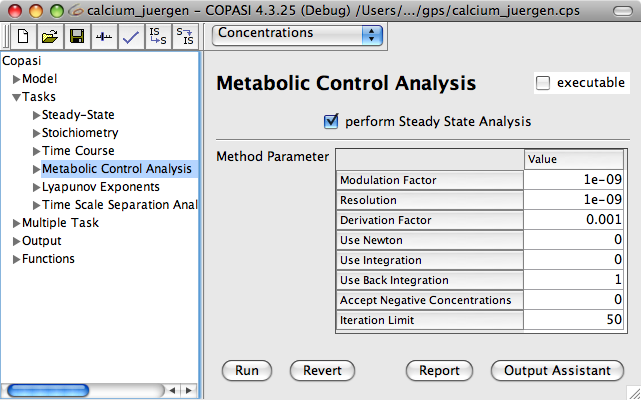
\includegraphics[scale=0.3]{images/MCATask_01.png}}}


In order to do a full MCA (elasticities and control coefficients), Copasi needs to look for a steady state first, otherwise Copasi can only calculate the elasticities. If you did not already \hyperlink{steadyStateAnalysis}{do a steady state calculation} right before so that the system already is in the steady state if one was found, you should enable the checkbox that tells Copasi to do a steady state calculation before calculating the MCA. Depending on wether Copasi needs to do a steady state analysis or not, you can change one or more parameters that influence the way the MCA and the steady state are calculated. The parameters for the steady state calculation or the same as for the steady state widget explained in the \hyperlink{steadyStateAnalysis}{{[Doing a Steady State Analysis]}} section. 


{{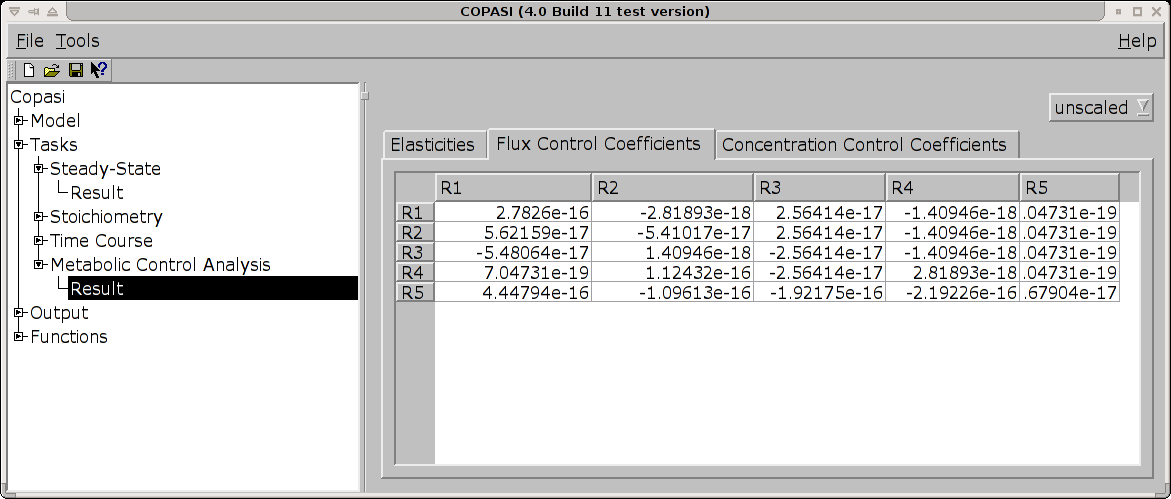
\includegraphics[scale=0.3]{images/MCATask_02.png}}}


To start the calculation, you click the {\sffamily \bfseries run} button. After the calculation is finished, Copasi will automatically switch to the results dialog. The results dialog shows three tabs that contain the results for the elasticities, flux control coefficients and concentration control coefficients.


{{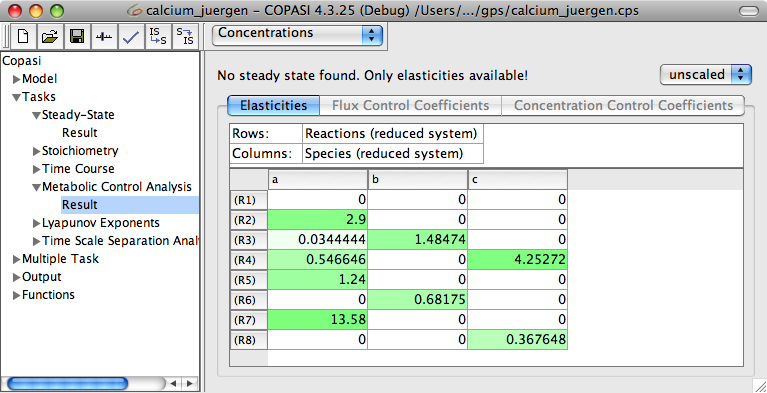
\includegraphics[scale=0.3]{images/MCATask_03.png}}}


Depending on wether a steady state was found or not, only the elasticities tab might be enabled. Copasi will state that it could not find a steady state in a label right above the tabs. For all of the results, you can choose if you want Copasi to display them scaled or unscaled.

% ------------------------   
% Section 
\section{Defining and Using Sliders}
\label{usingSliders}\hypertarget{usingSliders}{}%

Starting with Copasi Build 11 sliders to change parameter values interactively are available, but so far they are only available for the time course task.

Per default, the slider dialog is hidden, if you want it to be displayed, you have to activate it by toggling the corresponding menu entry in the {\sffamily \bfseries tools} menu. Depending on what element is selected in the object tree, the dialog will be disabled. If you select a task (or an element below the task) that supports sliders, the dialog will be enabled and display the sliders that are defined for this task.


{{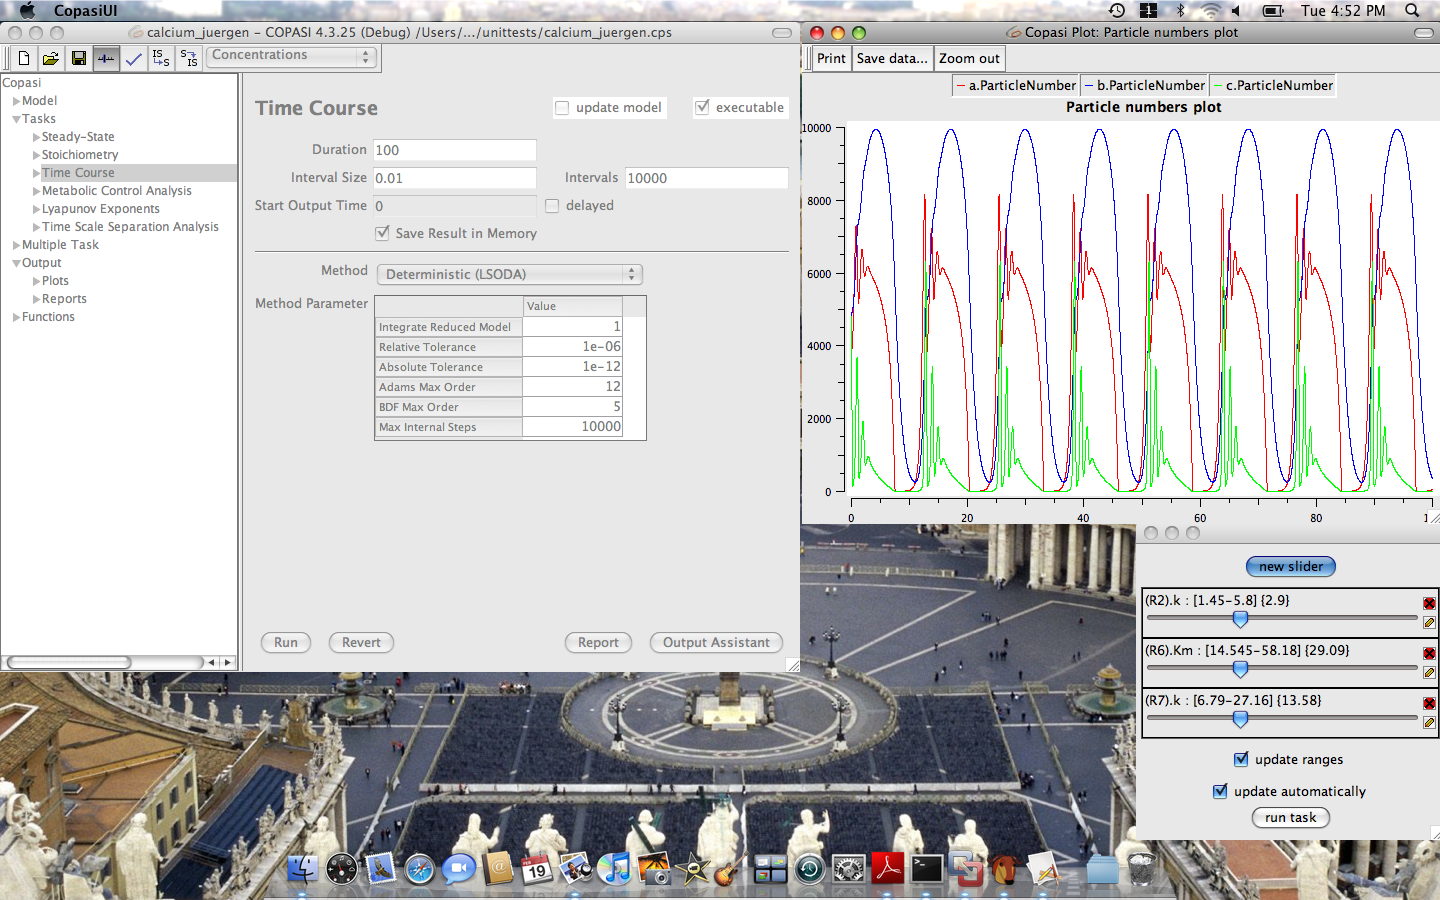
\includegraphics[scale=0.3]{images/Sliders_01.png}}}


If the sliders dialog is active, you can now add and modify existing sliders via a context menu. The context menu can be activated with the right mouse button (CTRL + Mouse button for single button mice on Macs!). If you right click on an existing slider, the menu will offer the possibilities to {\sffamily \bfseries delete} this slider or to {\sffamily \bfseries edit} it. If you right click into the dialog window where there is no slider, you will be offered the possility to define a new slider.


{{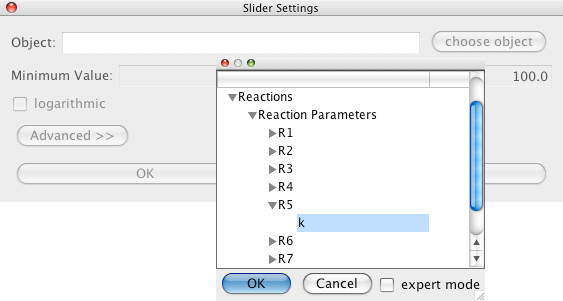
\includegraphics[scale=0.3]{images/Sliders_02.png}}}


Once you are in the dialog for the definition of a new slider, you have to choose an object to manipulate via the slider. This object can be selected from the selection dialog that pops up when you click on the {\sffamily \bfseries choose object} button. The selection tree is the same as the ones you get when \hyperlink{plotDefinitions}{selecting objects for a plot}. The selection dialog also offers an expert mode in case the object you want to manipulate with the slider is not present in the simplified tree. Usually the objects that you want to modify in the time course simulation are one or several of the reaction parameters. This way you can interactively see how the behavior of your model changes when you change a specific parameter. In combination with plots this is a very powerful way to examine the behavior of your model.

Once you have selected an object, you can set the parameters for the slider. You specify the range the slider has to cover in the {\sffamily \bfseries Minimum Value} and {\sffamily \bfseries Maximum Value} fields. The {\sffamily \bfseries Object Value} field determines the current value of the object that is associated with the slider. In the {\sffamily \bfseries Number of minor ticks} field you specify how many minor ticks your slider will have. And in the {\sffamily \bfseries Ticksize factor} field you specify how many minor ticks make a major tick. Major ticks can be used to coarsely go through the range of the slider wheras minor ticks allow you to step through the range in a more fine grained fashion. Instead of specifying the number of minor ticks, you can specify the size of a minor tick. If you change either of those two values, the other one will be adjusted accordingly. The formula is   \begin{displaymath}{\textrm{minor tick size}{ {\left( {\textrm{Maximum Value}-\textrm{Minimum Value}} \right)} /\textrm{number of minor ticks}}}\end{displaymath}%
  . Once you have made all the settings, you confirm the slider definfinition with the {\sffamily \bfseries OK} button. A new slider should appear in the slider dialog.


{{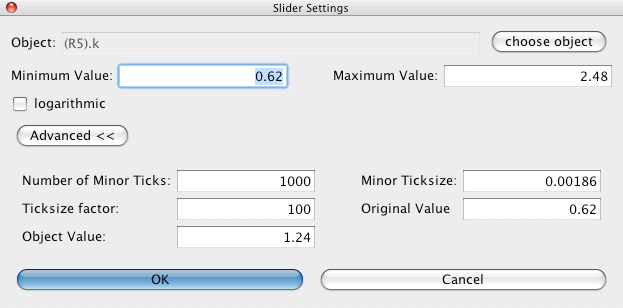
\includegraphics[scale=0.3]{images/Sliders_03.png}}}


Each slider shows the name of the object, the current value and the range in its label. The slider dialog has a checkbox called {\sffamily \bfseries update automaticaly} if this box is checked, Copasi will run the corresponding task each time you release a slider handle after moving it. If you don't want Copasi to automatically run the task each time you change a sliders value, you can uncheck this box and run the task manually by clicking on the {\sffamily \bfseries run task} button.

Modifying a slider is essentially the same as defining a slider. The only difference being that you can not change the object the slider is connceted to. In order to do that, you have to delete the slider and define a new slider for the new object.

% ------------------------   
% Section 
\section{Using the Tutorial Wizard}
\label{tutorialWizard}\hypertarget{tutorialWizard}{}%

Copasi also includes a short tutorial on how you create a model and run a time course simulation with plotting. You can start the wizard from the {\sffamily \bfseries help} menu. The corresponding menu entry is called {\sffamily \bfseries Simple Wizard}.


{{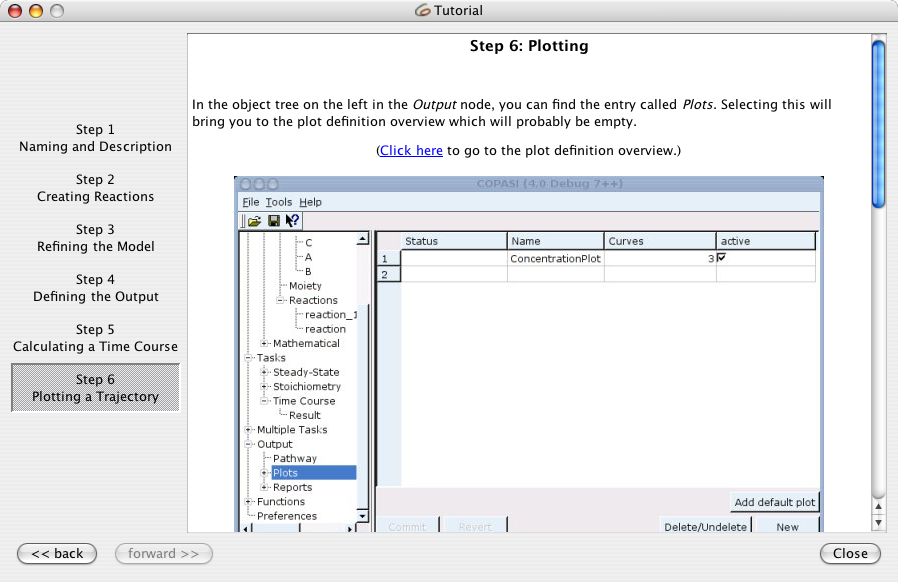
\includegraphics[scale=0.3]{images/Wizard_01.png}}}


The wizard leads you in six steps from creating a model to doing a time course simulation of the model and plotting the results of the time course.

On the left side of the wizard there are six buttons that correspond to the six steps. When you first open the wizard, step one is selected and the widget on the right shows some documentation that you should read and possibly repeat the steps explained. Once you are finished with step 1, you can either click directly on the button that corresponds to step 2, or you can click the {\sffamily \bfseries forward} button which will always bring you to the next step. If you would like to reread something from an earlier step, you can move to the specific step with the buttons or use the {\sffamily \bfseries forward} and {\sffamily \bfseries backward} buttons to navigate.

% ------------------------   
% Section 
\section{Importing and Exporting SBML Files}
\label{importExport}\hypertarget{importExport}{}%

Copasi is able to import SBML {\textless}\url{http://www.sbml.org}{\textgreater} level 1 and level 2 files as well as export SBML level 2 files through the corresponding entries in the {\sffamily \bfseries File} menu. For the import and export the SBML Model read with libsbml {\textless}\url{http://www.sbml.org/libsbml.html}{\textgreater} is converted to the Copasi model structure and vice versa.

On exporting, Copasi converts its native model structure to an sbml model that is again written out using libsbml. Since the SBML model structure is converted into the Copasi model structure upon import, some of the information in the SBML file gets lots because Copasi does not support the corresponding model elements. Examples of data that gets lost are rules and events. Also all annotations get lost.

Likewise, SBML does not support all of the elements of a Copasi model so some information from the Copasi model also gets lost when exporting an SBML file. For example task, reports and plot definitions are not exported to SBML.

This is normaly not a big problem since the essential parts of a model normaly get imported or exported. A consequence however one should keep in mind is that if you import an SBML file into Copasi and later export it again, it might have lost some of the original information. So if your SBML model depends on rules and events, it is not suitable for import into Copasi, although this might change in the future.

Copasi sometimes will also refuse to import "incomplete" SBML files, e.g. if one or more reaction do not contain a kinetic law. This is being worked on, but you should still be aware of the fact that Copasi sometimes refuses to load a perfectly valid SBML file.

\end{document}

